%
% Template Laporan Skripsi/Thesis 
%
% @author  Andreas Febrian, Lia Sadita 
% @version 1.03
%
% Dokumen ini dibuat berdasarkan standar IEEE dalam membuat class untuk 
% LaTeX dan konfigurasi LaTeX yang digunakan Fahrurrozi Rahman ketika 
% membuat laporan skripsi. Konfigurasi yang lama telah disesuaikan dengan 
% aturan penulisan thesis yang dikeluarkan UI pada tahun 2008.
%

%
% Tipe dokumen adalah report dengan satu kolom. 
%
\documentclass[12pt, a4paper, onecolumn, oneside, final]{report}

% Load konfigurasi LaTeX untuk tipe laporan thesis
\usepackage{uithesis}
\usepackage{natbib}
\usepackage{import}
% Load konfigurasi khusus untuk laporan yang sedang dibuat
%-----------------------------------------------------------------------------%
% Informasi Mengenai Dokumen
%-----------------------------------------------------------------------------%
% 
% Judul laporan. 
\var{\judul}{Judul Sesuatu Banget \f{English} Miring Juga}
% 
% Tulis kembali judul laporan, kali ini akan diubah menjadi huruf kapital
\Var{\Judul}{JUDUL SESUATU BANGET \f{ENGLISH} MIRING JUGA}
% 
% Tulis kembali judul laporan namun dengan bahasa Ingris
\var{\judulInggris}{Sesuatu Banget in English}

% 
% Tipe laporan, dapat berisi Skripsi, Tugas Akhir, Thesis, atau Disertasi
\var{\type}{Skripsi}
% 
% Tulis kembali tipe laporan, kali ini akan diubah menjadi huruf kapital
\Var{\Type}{Skripsi}
% 
% Tulis nama penulis 
\var{\penulis}{Ardhi Putra Pratama}
% 
% Tulis kembali nama penulis, kali ini akan diubah menjadi huruf kapital
\Var{\Penulis}{Ardhi Putra Pratama}
% 
% Tulis NPM penulis
\var{\npm}{0906562770}
% 
% Tuliskan Fakultas dimana penulis berada
\Var{\Fakultas}{Ilmu Komputer}
\var{\fakultas}{Ilmu Komputer}
% 
% Tuliskan Program Studi yang diambil penulis
\Var{\Program}{Ilmu Komputer}
\var{\program}{Ilmu Komputer}
\var{\programEng}{Computer Science}
% 
% Tuliskan tahun publikasi laporan
\Var{\bulanTahun}{Juli 2013}
% 
% Tuliskan gelar yang akan diperoleh dengan menyerahkan laporan ini
\var{\gelar}{Sarjana Ilmu Komputer}
% 
% Tuliskan tanggal pengesahan laporan, waktu dimana laporan diserahkan ke 
% penguji/sekretariat
\var{\tanggalPengesahan}{21 Juni 2013} 
% 
% Tuliskan tanggal keputusan sidang dikeluarkan dan penulis dinyatakan 
% lulus/tidak lulus
\var{\tanggalLulus}{5 Juli 2013}
% 
% Tuliskan pembimbing 
\var{\pembimbing}{Prof. Saya }
\var{\pembimbingdua}{Dia S.Kom, M.Kom}
% 
% Alias untuk memudahkan alur penulisan paa saat menulis laporan
\var{\saya}{Penulis}

%-----------------------------------------------------------------------------%
% Judul Setiap Bab
%-----------------------------------------------------------------------------%
% 
% Berikut ada judul-judul setiap bab. 
% Silahkan diubah sesuai dengan kebutuhan. 
% 
\Var{\kataPengantar}{Kata Pengantar}
\Var{\babSatu}{Pendahuluan}
\Var{\babDua}{Tinjauan Pustaka}
\Var{\babTiga}{Aplikasi Yang Digunakan}
\Var{\babEmpat}{Perancangan Implementasi dan Analisis}
\Var{\babLima}{Implementasi dan Pengujian}
\Var{\babEnam}{Hasil Implementasi dan Evaluasi}
\Var{\babTujuh}{Kesimpulan dan Saran}

% Daftar pemenggalan suku kata dan istilah dalam LaTeX
%
% Hyphenation untuk Indonesia 
%
% @author  Andreas Febrian
% @version 1.00
% 
% Tambahkan cara pemenggalan kata-kata yang salah dipenggal secara otomatis 
% oleh LaTeX. Jika kata tersebut dapat dipenggal dengan benar, maka tidak 
% perlu ditambahkan dalam berkas ini. Tanda pemenggalan kata menggunakan 
% tanda '-'; contoh:
% menarik
%   --> pemenggalan: me-na-rik
%

\hyphenation{
    % alphabhet A
    a-na-li-sa a-tur 
    a-pli-ka-si 
    % alphabhet B
    ba-ngun-an 
    be-be-ra-pa 
    ber-ge-rak
    ber-ke-lan-jut-an 
    ber-pe-nga-ruh 
    % alphabhet C
    ca-ri
    % alphabhet D
    di-ban-ding-kan
    di-de-fi-ni-si-kan
    di-ha-rap-kan
    di-ka-te-go-ri-kan
    di-mi-li-ki-nya
    di-se-rah-kan
    di-sim-pan di-pim-pin de-ngan da-e-rah di-ba-ngun da-pat di-nya-ta-kan 
    di-sim-bol-kan di-pi-lih di-li-hat de-fi-ni-si
    di-se-su-ai-kan
    % alphabhet E
    e-le-men
    e-ner-gi eks-klu-sif
    % alphabhet F
    fa-si-li-tas
    % alphabhet G
    ga-bung-an ge-rak
    % alphabhet H
    ha-lang-an
    he-te-ro-gen
    % alphabhet I
    i-ngin
    % alphabhet J
    % alphabhet K
    ke-hi-lang-an
    ku-ning 
    kua-li-tas ka-me-ra ke-mung-kin-an ke-se-pa-ham-an
    ke-te-pat-an
    kon-fi-gu-ra-si
    % alphabhet L
    ling-kung-an
    % alphabhet M
    me-min-ta
    me-mo-del-kan
    me-mo-ri
    men-de-fi-ni-si-kan
    me-neng-ah
    meng-a-tas-i me-mung-kin-kan me-nge-na-i me-ngi-rim-kan 
    meng-u-bah meng-a-dap-ta-si me-nya-ta-kan mo-di-fi-ka-si
    meng-a-tur
    meng-au-to-ma-si
    meng-a-ko-mo-da-si
    me-ngo-rek-si
    % alphabhet N
    nya-ta non-eks-klu-sif
    % alphabhet O
    % alphabhet P
    pa-ra-lel
    peng-ala-mat-an
    pen-ting
    penga-da-an
	pe-nye-rap-an 
	pe-ngon-trol
    pe-mo-del-an
    pe-ran  pe-ran-an-nya
    pe-rin-tah
    pem-ba-ngun-an pre-si-den pe-me-rin-tah prio-ri-tas peng-am-bil-an 
    peng-ga-bung-an pe-nga-was-an pe-ngem-bang-an 
    pe-nga-ruh pa-ra-lel-is-me per-hi-tung-an per-ma-sa-lah-an 
    pen-ca-ri-an peng-struk-tur-an
    pe-ner-bang-an
    pro-se-sor
    % alphabhet Q
    % alphabhet R
    ran-cang-an
    % alphabhet S
    se-dang-kan
    se-ring
    si-mu-la-si sa-ngat    
    % alphabhet T
    te-ngah
    ter-da-pat
    % alphabhet U
    u-sa-ha
    % alphabhet V
    % alphabhet W
    % alphabhet X
    % alphabhet Y
    % alphabhet Z
    % special
}
% Daftar istilah yang mungkin perlu ditandai 
%
% @author  Andreas Febrian
% @version 1.00
% 
% Mendaftar seluruh istilah yang mungkin akan perlu dijadikan 
% italic atau bold pada setiap kemunculannya dalam dokumen. 
% 

\var{\license}{\f{Creative Common License 1.0 Generic}}
\var{\bslash}{$\setminus$}


%\usepackage[backend=bibtex]{biblatex}
%\addbibresource{bib.bib}

% Awal bagian penulisan laporan
\begin{document}
%
% Sampul Laporan
%%
% Sampul Laporan

%
% @author  unknown
% @version 1.01
% @edit by Andreas Febrian
%

\begin{titlepage}
    \begin{center}    
        \begin{figure}
            \begin{center}
                
\includegraphics[width=2.5cm]{pics/makara.png}
            \end{center}
        \end{figure}    
        \vspace*{0cm}
        \bo{
        	UNIVERSITAS INDONESIA\\
        }
        
        \vspace*{1.0cm}
        % judul thesis harus dalam 14pt Times New Roman
        \bo{\Judul} \\[1.0cm]

        \vspace*{2.5 cm}    
        % harus dalam 14pt Times New Roman
        \bo{\Type}

        \vspace*{3 cm}       
        % penulis dan npm
        \bo{\Penulis} \\
        \bo{\npm} \\

        \vspace*{5.0cm}

        % informasi mengenai fakultas dan program studi
        \bo{
        	FAKULTAS \Fakultas\\
        	PROGRAM STUDI \Program \\
        	DEPOK \\
        	\bulanTahun
        }
    \end{center}
\end{titlepage}


%
% Gunakan penomeran romawi
\pagenumbering{roman}

%
% load halaman judul dalam
\addChapter{HALAMAN JUDUL}
%%
% Halaman Judul Laporan 
%
% @author  unknown
% @version 1.01
% @edit by Andreas Febrian
%

\begin{titlepage}
    \begin{center}\begin{figure}
            \begin{center}
                
\includegraphics[width=2.5cm]{pics/makara.png}
            \end{center}
        \end{figure}    
        \vspace*{0cm}
        \bo{
        	UNIVERSITAS INDONESIA\\
        }
        
        \vspace*{1.0cm}
        % judul thesis harus dalam 14pt Times New Roman
        \bo{\Judul} \\[1.0cm]

        \vspace*{2.5 cm}    
        % harus dalam 14pt Times New Roman
        \bo{\Type} \\
        % keterangan prasyarat
        \bo{Diajukan sebagai salah satu syarat untuk memperoleh gelar \\
        \gelar}\\

        \vspace*{3 cm}       
        % penulis dan npm
        \bo{\Penulis} \\
        \bo{\npm} \\

        \vspace*{5.0cm}

        % informasi mengenai fakultas dan program studi
        \bo{
        	FAKULTAS \Fakultas\\
        	PROGRAM STUDI \Program \\
        	DEPOK \\
        	\bulanTahun
        }
    \end{center}
\end{titlepage}

%
% setelah bagian ini, halaman dihitung sebagai halaman ke 2
\setcounter{page}{2}

% sementara ga usah
% load halaman pengesahan
%\addChapter{LEMBAR PERSETUJUAN}
%%
% Halaman Pengesahan
%
% @author  Andreas Febrian
% @author  Ardhi Putra Pratama
% @version 1.1
%

\chapter*{HALAMAN PERSETUJUAN}

\vspace*{0.2cm}
\noindent 

\noindent
\begin{tabular}{l l p{11cm}}
	\bo{Judul}&: & \judul \\ 
	\bo{Nama}&: & \penulis \\
	\bo{NPM}&: & \npm \\
\end{tabular} \\

\vspace*{1.2cm}


\noindent\begin{minipage}[b]{0.6\hsize}
  \raggedright
  Laporan \type~ini telah diperiksa dan disetujui.\\[0.3cm]
  
  \tanggalPengesahan \\[2cm]
  
  \underline{\pembimbing}\\[0.1cm]
  Pembimbing \type
\end{minipage}
\hfill
\begin{minipage}[b]{0.4\hsize}
  \raggedleft
  .\\[2cm]
  \underline{\pembimbingdua}\\[0.1cm]
  Pembimbing \type
\end{minipage}

\newpage
%
% load halaman orisinalitas 
\addChapter{LEMBAR PERNYATAAN ORISINALITAS}
%%
% Halaman Orisinalitas
%
% @author  Andreas Febrian
% @version 1.01
%

\chapter*{\uppercase{halaman pernyataan orisinalitas}}
\vspace*{2cm}

\begin{center}
	\bo{\type~ini adalah hasil karya saya sendiri, \\ 
	dan semua sumber baik yang dikutip maupun dirujuk \\
	telah saya nyatakan dengan benar.} \\
	\vspace*{2.6cm}
	
	\begin{tabular}{l c l}
	\bo{Nama} & : & \bo{\penulis} \\
	\bo{NPM} & : & \bo{\npm} \\ 
	\bo{Tanda Tangan} & : & \\
	& & \\
	& & \\
	\bo{Tanggal} & : & \bo{\tanggalPengesahan} \\	
	\end{tabular}
\end{center}

\newpage
%
%
\addChapter{LEMBAR PENGESAHAN}
%%
% Halaman Pengesahan Sidang
%
% @author  Andreas Febrian, Andre Tampubolon 
% @version 1.02
%

\chapter*{HALAMAN PENGESAHAN}

\vspace*{0.4cm}
\noindent 

\noindent
\begin{tabular}{ll p{9cm}}
	\type~ini diajukan oleh&: & \\
	Nama&: & \penulis \\
	NPM&: & \npm \\
	Program Studi&: & \program \\
	Judul \type&: & \judul \\
\end{tabular} \\

\vspace*{1.0cm}

\noindent \bo{Telah berhasil dipertahankan di hadapan Dewan Penguji 
dan diterima sebagai bagian persyaratan yang diperlukan untuk 
memperoleh gelar \gelar~pada Program Studi \program, Fakultas 
\fakultas, Universitas Indonesia.}\\[0.2cm]

\begin{center}
	\bo{DEWAN PENGUJI}
\end{center}

\vspace*{0.3cm}

\begin{tabular}{l l l l }
	& & & \\
	Pembimbing&: & \pembimbing & (\hspace*{3.0cm}) \\
	& & & \\
	Pembimbing&: & \pembimbingdua & (\hspace*{3.0cm}) \\
	& & & \\
	Penguji&: & Penguji 1 & (\hspace*{3.0cm}) \\
	& & & \\
	Penguji&: & Penguji 2 & (\hspace*{3.0cm}) \\
\end{tabular}\\

\vspace*{2.0cm}

\begin{tabular}{ll l}
	Ditetapkan di&: & Depok\\
	Tanggal&: & \tanggalLulus \\
\end{tabular}


\newpage
%
%
\addChapter{\kataPengantar}
%%-----------------------------------------------------------------------------%
\chapter*{\kataPengantar}
%-----------------------------------------------------------------------------%
Puji dan syukur kehadirat Tuhan Yang Maha Esa karena hanya dengan rahmat-Nya, penulis dapat menyelesaikan pembuatan skripsi ini. Penulisan skripsi ini ditujukan untuk memenuhi salah satu syarat untuk menyelesaikan pendidikan pada Program Sarjana, Universitas Indonesia. Selama menempuh kegiatan penerimaan dan adaptasi, belajar-mengajar, hingga penulisan skripsi ini, tidaklah dilakukan sendirian. Untuk itu, Saya ingin berterima kasih kepada berbagai pihak yang telah membantu, mendampingi, dan mendapingi, diantaranya adalah:

\begin{enumerate}
  \item Kedua orang tua, serta kakak dan adik yang selalu memberikan dukungan dan doa.
  \item Dra. Mirna Adriani, Ph.D. dan Rahmad Mahendra, S.Kom., M.Sc. selaku dosen pembimbing yang banyak memberikan arahan, masukan, dan bantuan dalam menyelesaikan skripsi ini.
  \item Teman-teman Lab Information Retrieval (Ilham Fathy, Valdi Rachman, Karunia, Aldi, Christian Halim, Saga, Dhanang), sebagai rekan yang telah berbagi ilmu, saran, dan motivasi.
  \item Segenap teman-teman angkatan 2013 (Angklung) yang memberi dukungan dan semangat untuk menyelesaikan skripsi ini.
  \item Teman-teman anotator (Niken, Yola, Rahmi, Jundi, Meuthia, Amel) yang telah membantu dalam tahap pengerjaan skripsi ini.
  \item Pihak-pihak lain yang tidak dapat disebutkan satu-persatu yang sudah memberikan bantuan dan dukungan.
\end{enumerate}

\vspace*{0.1cm}
\begin{flushright}
Depok, 5 Juni 2017\\[0.1cm]
\vspace*{1cm}
\penulis

\end{flushright}

%
%
\addChapter{LEMBAR PERSETUJUAN PUBLIKASI ILMIAH}
%% 
% @author  Andre Tampubolon, Andreas Febrian
% @version 1.01
% 

\chapter*{\uppercase{Halaman Pernyataan Persetujuan Publikasi Tugas Akhir untuk Kepentingan Akademis}}

\vspace*{0.2cm}
\noindent 
Sebagai sivitas akademik Universitas Indonesia, saya yang bertanda 
tangan di bawah ini:
\vspace*{0.4cm}


\begin{tabular}{p{4.2cm} l p{6cm}}
	\bo{Nama} & : & \penulis \\ 	
	\bo{NPM} & : & \npm \\
	\bo{Program Studi} & : & \program\\	
	\bo{Fakultas} & : & \fakultas\\
	\bo{Jenis Karya} & : & \type \\
\end{tabular}

\vspace*{0.6cm}
\noindent demi pengembangan ilmu pengetahuan, menyetujui untuk memberikan 
kepada Universitas Indonesia \bo{Hak Bebas Royalti Noneksklusif 
(Non-exclusive Royalty Free Right)} atas karya ilmiah saya yang berjudul:
\begin{center}
	\judul
\end{center}
beserta perangkat yang ada (jika diperlukan). Dengan Hak Bebas Royalti 
Noneksklusif ini Universitas Indonesia berhak menyimpan, 
mengalih media/formatkan, mengelola dalam bentuk pangkalan data 
(\f{database}), merawat, dan memublikasikan tugas akhir saya selama 
tetap mencantumkan nama saya sebagai penulis/pencipta dan sebagai 
pemilik Hak Cipta. \\

\noindent Demikian pernyatan ini saya buat dengan sebenarnya.

\begin{center}
	\vspace*{0.8cm}
	\begin{tabular}{lll}
		Dibuat di&: & Depok \\
		Pada tanggal&: & \tanggalPengesahan \\
	\end{tabular}\\

	\vspace*{0.2cm}
	Yang menyatakan \\
	\vspace*{2cm}
	(\penulis)
\end{center}

\newpage


%
% 
\singlespacing
\addChapter{ABSTRAK}
%%
% Halaman Abstrak
%
% @author  Andreas Febrian
% @version 1.00
%

\chapter*{Abstrak}

\vspace*{0.2cm}

\noindent \begin{tabular}{l l p{10cm}}
	Nama&: & \penulis \\
	Program Studi&: & \program \\
	Judul&: & \judul \\
\end{tabular} \\ 

\vspace*{0.5cm}

\noindent 
\\ lalalalala

\vspace*{0.2cm}

\noindent Kata Kunci: \\ 
\noindent relasi kata, \textit{pattern}, \textit{semi-supervised}, hipernim-hiponum\\ 

\newpage

%
%
%%
% Halaman Abstract
%
% @author  Andreas Febrian
% @version 1.00
%

\chapter*{ABSTRACT}

\vspace*{0.2cm}

\noindent \begin{tabular}{l l p{11.0cm}}
	Name&: & \penulis \\
	Program&: & \programEng \\
	Title&: & \judulInggris \\
\end{tabular} \\ 

\vspace*{0.5cm}

\noindent 
\\ Word relation extraction is one of research branch in Natural Language Processing (NLP) which purpose is to extract words based on the defined relations. Corpus that holds the relationship among words is used for other future research. For English, those corpus can be found in one of the famous digital dictionary which is WordNet. Unfortunatelly, the current WordNet Bahasa Indonesia is not perfect and still contains errors. This research aims to automatically build a semantically related words corpus for Bahasa Indonesia. Many other researches had been done before with various methods. In this research, pattern analysis aproach was used which consists of pattern extraction and pattern matching. The corpus was build gradually using semi-supervised learning. The relation that was observed is semantic relation hypernym and hyponym and this research used Wikipedia as the datasource. At the end of this research, a corpus which contains 3493 pair of related words had successfully been built. The accuracy for every experiments were above 0.80. Those infomations show that using pattern analysis to extract pair of related words from Wikipedia has a potential to be used for gathering large sum of data and having good quality.

\vspace*{0.2cm}

\noindent Keywords: \\ 
\noindent  word relation, pattern extraction, pattern matching, semi-supervised, hypernym, hyponym, corpus \\
\newpage


%
% Daftar isi, gambar, dan tabel
%
%\tableofcontents
%\clearpage
%\listoffigures
%\clearpage
%\listoftables
%\clearpage
%\lstlistoflistings
%\clearpage

%
% Gunakan penomeran Arab (1, 2, 3, ...) setelah bagian ini.
%
\pagenumbering{arabic}

%
%
%
\onehalfspacing
%!TEX root = skripsi.tex
%-----------------------------------------------------------------------------%
\chapter{\babSatu}
%-----------------------------------------------------------------------------%
Bab ini membahas mengenai latar belakang penelitian, perumusan masalah, tujuan dan manfaat dilakukannya penelitian, ruang lingkup penelitan, dan terakhir metodologi yang digunakan. 


%-----------------------------------------------------------------------------%
%-----------------------------------------------------------------------------%
\section{Latar Belakang}
%-----------------------------------------------------------------------------%
Relasi kata adalah informasi mengenai hubungan yang dimiliki antar satu kata dengan kata yang lain. Informasi tersebut sering digunakan untuk menunjang berbagai penelitian, salah satunya adalah \textit{Question Answering} atau sistem tanya jawab. Suatu pertanyaan dapat langsung dijawab jika diketahui hubungan antar suatu kata dalam pertanyaan dengan relasi yang ditanyakan. Sebagai contoh jika diberi pertanyaan `Apa ibu kota Indonesia?' dan dimiliki suatu \textit{resource} yang menyimpan relasi ibu-kota(Indonesia, Jakarta) maka pertanyaan tersebut langsung dapat dijawab dengan jawaban `Jakarta'.

Salah satu subbagian dalam proses pengembangan sistem tanya jawab tersebut adalah \textit{answer type detection} yang berusaha untuk mencari tahu tipe jawaban sehingga dapat menurunkan lama proses pencarian \citep{jurafsky2000speech}. Tipe jawaban dapat dibangun dalam bentuk hirarki atau yang dikenal sebagai \textit{answer type taxonomy}. Sebuah kata dalam pertanyaan mengandung informasi yang dapat mengenali tipe jawaban. Mengetahui hipernim dan hiponim kata tersebut dapat membantu mencari tahu tipe jawaban.

Berikut adalah beberapa contoh pertanyaan yang jawabannya dengan memanfaatkan informasi relasi semantik dari \textit{question headwords}-nya.

Q1. What are aquatic vertebrates?

Q2. Which type of cat that has short hair and blue eyes?

\noindent Pertanyaan pertama ingin mengetahui apa saja vertebrata yang hidup di air, sementara pertanyaan kedua ingin mengetahui jenis kucing yang berbulu pendek dan bermata biru. Pada pertanyaan pertama, \textit{question headword}-nya adalah `aquatic vertebrate'. Jika dilihat menggunakan salah satu kamus online populer, yaitu WordNet, dapat langsung diketahui jawabanya adalah `fish' (ikan) melalui relasi semantik yang dimiliki oleh kata tersebut. Untuk pertanyaan kedua dapat diketahui bahwa domain jawabanya merupakan `cat' (kucing) sehingga dapat langsung didaftar jenis kucing yang memiliki ciri-ciri yang sesuai. Hal tersebut memperlihatkan bahwa relasi semantik antar kata dibutuhkan untuk mempermudah penyelesaia masalah \textit{question answering}. 

Resource pasangan kata relasi semantik dalam Bahasa Inggris dapat diambil dari salah satu kamus digital populer yaitu WordNet \citep{miller1995wordnet}. WordNet tersebut dibangun secara manual oleh berbagai ahli linguistik. Setiap \textit{entry} pada WordNet disimpan dalam bentuk set sinonim atau biasa disebut \textit{synset} dan arti dari \textit{synset} tersebut atau biasa disebut \textit{sense}. \textit{Entry} dalam WordNet juga mengandung informasi mengenai relasi semantik antar \textit{synset}. Penelitian mengenai pembangunan WordNet Bahasa Indonesia telah dilakukan sebelumnya, sayangnya jumlah \textit{entry} dalam WordNet Bahasa Indonesia masih sangat terbatas. Selain itu, relasi semantik dalam WordNet juga belum dapat dikatakan baik. Mengetahui hal tersebut, penelitian ini berusaha membangun korpus pasangan kata relasi Behasa Indonesia.

Penelitian ini berusaha mengekstrak kata berdasarkan relasi tertentu dari suatu dokumen sehingga dihasilkan korpus pasanagan relasi kata. Fokus relasi dalam penelitian ini adalah relasi semantik hiperim-hiponim. Keduanya menyatakan relasi antara kata yang lebih umum (hipernim) dengan kata yang lebih khusus (hiponim). Berbagai penelitian sebelumnya sudah pernah mencoba mengekstrak relasi kata hipernim-hiponim dengan berbagai metode. Pada penelitian ini, metode yang digunakan adalah \textit{pattern extraction} dan \textit{matching} dengan memanfaatkan korpus Wikipedia Bahasa Indonesia. Wikipedia memuat banyak kata dari berbagai domain sehingga dapat dimanfaatkan untuk membuat \textit{pattern} yang general serta menghasilkan korpus berukuran besar.

% Berbagai penelitian yang berkaitan dengan \textit{Information Retrieval} dan \textit{Natural Language Processing} mulai muncul menggunakan Bahasa Indonesia. Salah satu yang Informasi mengenai kata dan artinya sangat dibutuhkan. Sayangnya, \textit{resource} yang dimiliki berbasis Bahasa Indonesia masih sangat terbatas. Informasi tersebut umumnya disimpan dalam kamus digital seperti WordNet. Penelitian ini dilaksanakan untuk mengembangkan \textit{resource} dalam Bahasa Indonesia. 

% WordNet adalah kamus digital yang dapat digunakan untuk menunjang penelitian di bidang \textit{Information Retrieval}dan \textit{Natural Language Processing}. WordNet yang paling sering digunakan dalam berbagai penelitian adalah WordNet Princeton berbahasa Inggris yang dibentuk secara manual oleh ahli linguistik. Setiap \textit{entry} pada WordNet disimpan dalam bentuk set sinonim atau biasa disebut \textit{synset} dan arti dari \textit{synset} tersebut atau biasa disebut \textit{sense}. Informasi lain yang disimpan dalam suatu synset adalah relasi antar synset. Relasi semantik yang tersimpan dalam WordNet adalah \textit{synonym}, \textit{antonym}, hipernim, hiponim, \textit{holonym}, \textit{meronym}, \textit{troponym}, dan \textit{entailment}.

% Beberapa penelitian telah dilakukan untuk membangun WordNet Bahasa Indonesia. WordNet Bahasa Indonesia yang telah ada adalah Indonesian WordNet (IWN) yang dibuat oleh Fakultas Ilmu Komputer Universitas Indonesia (Fasilkom UI) dan WordNet Bahasa yang dibuat oleh Nanyang Technology University (NTU). Salah satu kelemahan kedua WordNet tersebut adalah ukurannya yang masih sangat terbatas. Selain itu, informasi mengenai relasi kata juga belum dapat tersimpan secara baik. Kedua WordNet memetakan \textit{synset} Bahasa Indonesia ke WordNet Princeton dan memanfaatkan relasi yang di dalamnya. Mengetahui hal tersebut, dilakukan penelitian yang dapat mengekstrak relasi antar kata dengan hanya menggunakan korpus Bahasa Indonesia. Proses ekstraksi berjalan secara cepat dan data yang dihasilkan berjumlah besar. Korpus yang dihasilkan diharapkan dapat berguna untuk penelitian selanjutnya.

% Relasi kata adalah salah satu hal penting yang perlu diketahui jika ingin mengetahui hubungan antar kata secara semantik. Informasi yang berkaitan dengan semantik atau arti kata sulit diperoleh tanpa adanya pengetahuan sebelumnya. Kata-kata yang mirip secara leksikal belum tentu berelasi secara semantik. Sementara kata-kata yang tidak memiliki kesamaan secara leksikal bisa memiliki arti yang mirip atau berhubungan secara semantik. Korpus relasi yang dibuat diharapkan dapat membantu memperoleh informasi tersebut. Selain itu, pengetahuan mengenai relasi kata dapat dimaanfatkan dalam berbagai penelitian lain seperti \textit{question answering} \citep{ravichandran2002learning}, \textit{information extraction}, dan \textit{anaphora resolution}.

% Melihat adanya kebutuhan akan korpus relasi kata, dilakukanlah penelitian \textit{word relation extraction}. Penelitian ini berusaha mengekstrak kata berdasarkan relasi tertentu dari suatu dokumen sehingga dihasilkan korpus relasi kata. Penelitian kali ini akan fokus pada relasi kata \textit{hypernym-hyponym}. Keduanya menyatakan relasi antara kata yang lebih umum (hipernim) dengan kata yang lebih khusus (hiponim). Metode yang digunakan adalah pattern matching dengan memanfaatkan korpus Wikipedia Bahasa Indonesia. Wikipedia memuat banyak kata dari berbagai domain sehingga dapat dimanfaatkan untuk membuat pattern yang general serta menghasilkan korpus relasi berukuran besar.

%-----------------------------------------------------------------------------%
%-----------------------------------------------------------------------------%
\section{Perumusan Masalah}
%-----------------------------------------------------------------------------%
Berdasarkan latar belakang yang telah dipaparkan, pertanyaan yang menjadi rumusan penelitian adalah sebagai berikut.
\begin{enumerate}
	\item Bagaimana cara membangun korpus pasangan kata relasi hypernim-hiponim berkualitas baik secara otomatis?
	\item Seberapa baik metode \textit{pattern extraction} dan \textit{matching} digunakan untuk ekstraksi pasangan kata relasi semantik kata Bahasa Indonesia?
	% \item Bagaimana cara mengevaluasi \textit{pattern} dan korpus relasi kata dari hasil eksperimen?
\end{enumerate}

%-----------------------------------------------------------------------------%
%-----------------------------------------------------------------------------%
\section{Tujuan dan Manfaat Penelitian}
%-----------------------------------------------------------------------------%
Tujuan dari penelitian \textit{word relation extraction} ini adalah membangun korpus pasangan relasi semantik kata Bahasa Indonesia berukuran besar dan berkualitas baik secara otomatis. Selain itu, ingin diketahui pula apakah metode \textit{pattern extraction} dan \textit{matching} baik digunakan untuk mengekstrak relasi kata Bahasa Indonesia. Diharapkan korpus pasangan kata relasi yang dihasilkan dapat menunjang berbagai penelitian selanjutnya.

Penelitian ini juga diharapkan dapat memotivasi adanya penelitian selanjutnya di bidang \textit{Language Resource Development}, terutama pembangunan WordNet Bahasa Indonesia. Penelitian mengenai ekstraksi relasi kata berikutnya dengan berbagai metode lain diharapkan terus dilaksanakan sehingga Bahasa Indonesia memiliki \textit{resource} yang semakin baik.

%-----------------------------------------------------------------------------%
%-----------------------------------------------------------------------------%
\section{Ruang Lingkup Penelitian}
%-----------------------------------------------------------------------------%
Penelitian ini berupaya membangun korpus pasangan kata relasi semantik untuk Bahasa Indonesia. Relasi semantik yang menjadi fokus penelitian adalah hipernim dan hiponim, dengan kelas katanya yaitu \textit{noun} dan \textit{proper noun}. Penelitian ini berusaha mengekstrak tidak hanya kata-kata yang merupakan \textit{single token} seperti `komputer' dan `sekolah', namun juga kata-kata yang merupakan \textit{multi token} seperti `bulu tangkis' serta \textit{noun phrase} seperti `mamalia laut'.

% Penelitian ini hanya fokus pada pembuatan korpus pasangan kata dengan relasi hipernim dan hiponim Bahasa Indonesia. Kelas kata yang menjadi fokusi penelitan adalah kata benda (\textit{noun}). Pengembangan korpus dilakukan secara \textit{semi-supervised} dengan metode \textit{pattern matching}. \textit{Pattern} yang dibuat masih terbatas hanya merupakan \textit{pattern} leksikal. Evaluasi akan dilakukan pada \textit{pattern} dan korpus pasangan kata yang dihasilkan. Proses evaluasi korpus pasangan kata dilakukan menggunakan teknik \textit{random sampling}. Data yang digunakan untuk pembuatan \textit{pattern} maupun untuk ekstraksi korpus pasangan kata baru adalah Wikipedia Bahasa Indonesia. 
% Pemilihan relasi \textit{hypernym-hyponym} dalam penelitian karena memiliki berbagai manfaat. Relasi tersebut dapat mengidentifikasi \textit{Proper Noun} baru yang belum diketahui maknanya.

%-----------------------------------------------------------------------------%
%-----------------------------------------------------------------------------%
\section{Tahapan Penelitian}
%-----------------------------------------------------------------------------%
Proses penelitian dilakukan dalam beberapa tahapan sebagai berikut.
\begin{enumerate}
	\item Studi Literatur \\
	Pada tahap ini, dilakukan pembelajaran mengenai penelitian-penelitian sebelumnya yang telah dilakukan di bidang \textit{word relation extraction} sehingga diketahui langkah yang perlu diambil selanjutnya.
	\item Perumusan Masalah \\
	Perumusan masalah dilakukan untuk mendefinisikan masalah yang ingin diselesaikan, tujuan penelitian, dan hasil yang diharapkan sehingga proses penelitian dapat berjalan dengan baik.
	\item Rancangan Penelitian \\
	Setelah diketahui hasil yang ingin dicapai, dirancang tahap-tahap eksperimen secara terstruktur. Hal-hal yang diperhatikan mulai dari pengumpulan korpus awal (\textit{seed}), \textit{pre-processing} dokumen, perancangan implementasi \textit{pattern extraction} \textit{matching}, hingga proses evaluasi.
	\item Implementasi \\
	Implementasi dilaksanakan sesuai dengan rancangan penelitian untuk menjawab rumusan masalah. Segala hasil yang ditemukan digunakan untuk terus memperbaiki metode dan teknik penelitan sehingga didapatkan hasil yang semakin baik.
	\item Analisis dan Kesimpulan \\
	Tahap terakhir dari penelitian ini adalah menganalisis korpus pasangan kata relasi yang dihasilkan. Pertanyaan dari perumusan masalah dijawab, kemudian ditarik kesimpulan.
	
\end{enumerate}


-----------------------------------------------------------------------------%
\section{Sistematika Penulisan}
-----------------------------------------------------------------------------%
Sistematika penulisan laporan ini adalah sebagai berikut.
\begin{itemize}
	\item Bab 1 \babSatu \\
	Pada bab ini, dijelaskan latar belakang topik penelitian. Selain itu, perumusan masalah, tujuan penelitan, ruang lingkup penelitian, serta tahapan penelitan dipaparkan dalam bab ini.
	\item Bab 2 \babDua \\
	Bab ini memaparkan teori-teori dasar yang menjadi pedoman penelitian. Seluruh studi literatur mengenai teknik-teknik yang digunakan seperti \textit{pattern matching} dan \textit{extraction}, arsitektur \textit{semi-supervised}, metode evaluasi dan hal-hal mendasar lain yang berhubungan dengan penelitian ini.
	\item Bab 3 \babTiga \\
	\item Bab 4 \babEmpat \\
	\item Bab 5 \babLima \\
	\item Bab 6 \babEnam \\
\end{itemize}


%!TEX root = skripsi.tex
%-----------------------------------------------------------------------------%
\chapter{\babDua}
%-----------------------------------------------------------------------------%
Pada bab ini, dijelaskan mengenai studi literatur yang dilakukan. Studi literatur yang dilakukan digunakan sebagai dasar konsep dan teknik penelitian. Dipaparkan pula berbagai istilah dan metode yang digunakan dalam penelitian.


%-----------------------------------------------------------------------------%
\section{WordNet}
%-----------------------------------------------------------------------------%
WordNet adalah kamus leksikal yang tersimpan secara digital dan digunakan untuk berbagai keperluan komputasi \citep{miller1995wordnet}. Pembuatan WordNet dilatarbelakangi keperluan mendapatkan \textit{sense} atau arti semantik suatu kata. Informasi tersebut perlu disimpan dan dapat dibaca oleh mesin. WordNet pertama dibuat oleh \cite{miller1995wordnet} berbasis Bahasa Inggris dan sekarang dikenal dengan nama Princeton WordNet (PWN). WordNet menyimpan informasi dalam bentuk database dimana setiap entry-nya adalah pasangan \textit{synset} dan arti semantiknya (\textit{sense}). Set sinonim (\textit{synset}) adalah himpunan kata yang memiliki arti yang sama atau saling berelasi \textit{synonym}. 

WordNet mengandung beberapa kelas kata seperti kata benda (\textit{noun}), kata kerja (\textit{verb}), kata sifat (\textit{adjective}), dan kata keterangan (\textit{adverb}). WordNet juga menyimpan informasi mengenai relasi semantik antar \textit{synset}. Relasi yang disimpan adalah \textit{synonymy}, \textit{antonymy}, \textit{hyponymy}, \textit{hypernym}, \textit{meronymy}, \textit{holonymy}, \textit{troponymy}, dan \textit{entailment}.

%-----------------------------------------------------------------------------%
\subsection{Indonesian WordNet}
%-----------------------------------------------------------------------------%
Penelitian mengenai WordNet Bahasa Indonesia pernah dilakukan sebelumnya oleh \cite{putra2008building} dan \cite{margaretha2008comparing}. Indonesian WordNet (IWN) dibangun menggunakan metode mapping antara WordNet yang sudah ada ke dalam Bahasa Indonesia \citep{putra2008building}. WordNet yang digunakan sebagai dasarnya adalah Princeton WordNet. Synset dalam PWN akan dipetakan ke dalam entry Kamus Besar Bahasa Indonesia (KBBI), sehingga menghasilkan hasil yang berkualitas baik secara cepat dan mudah. Penelitian tersebut menghasilkan 1441 synset dan 3074 sense. Relasi semantik antar synset diperoleh dengan memetakan IWN synset dengan PWN synset, sehingga relasi yang dimiliki dalam PWN dapat diturunkan.

%-----------------------------------------------------------------------------%
\subsection{WordNet Bahasa}
%-----------------------------------------------------------------------------%
Pengembangan WordNet untuk Bahasa Indonesia juga dilakukan oleh Nanyang Technology University (NTU) sejak tahun 2011 dan diberi nama WordNet Bahasa \citep{noor2011creating}. WordNet ini telah diintegrasi dengan salah satu \textit{tools} NLP berbasis Python yaitu nltk sehingga dapat dengan mudah digunakan dalam komputasi. WordNet Bahasa juga memanfaatkan PWN untuk mendapatkan relasi semantik antar \textit{synset}. Pada penelitian ini, dimanfaatkan \textit{tools} tersebut untuk mendapatkan \textit{seed} relasi semantik antar kata dalam Bahasa Indonesia.

%-----------------------------------------------------------------------------%
\subsection{Kelemahan WordNet Bahasa Indonesia}
%-----------------------------------------------------------------------------%
Hingga saat ini, relasi semantik antar kata yang dimiliki oleh WordNet Bahasa Indonesia merupakan hasil turunan dari relasi semantik WordNet Princeton. Sayangnya, pemanfaatan PWN untuk mendapatkan relasi semantik kata Bahasa Indonesia menemui beberapa hambatan. WordNet Bahasa Indonesia menjadi sangat tergantung dengan struktur PWN untuk mendapatkan relas semantik suatu \textit{synset}. Selain itu, beberapa \textit{synset} Bahasa Indonesia juga tidak dapat dipetakan secara tepat ke \textit{synset} PWN, beberapa kata kehilangan arti atau mendapat arti yang kurang tepat. Hal ini menyebabkan pasangan kata relasi semantik Bahasa Indonesia yang dihasilkan terlihat kurang baik. Untuk itu, dicetuskanlah penelitian untuk mengekstrak relasi semantik dalam Bahasa Indonesia secara mandiri. 


%-----------------------------------------------------------------------------%
\section{Relasi}
%-----------------------------------------------------------------------------%
Relasi menggambarkan hubungan atau koneksi yang dimiliki oleh suatu hal dengan yang lain (KBBI). Dalam bidang matematika, relasi memetakan suatu anggota dari himpunan satu ke himpunan lain sesuai dengan hubungan yang didefinisikan. Dalam penelitian ini, relasi yang diperhatikan adalah relasi semantik antar kata. Domainnya adalah kata-kata yang tergabung dalam kelas kata benda (\textit{noun}).

Satu relasi dapat terdiri dari beberapa entitas dan dituliskan dalam bentuk tuple $t = (e_1, e_2, ..., e_n)$ dimana $e_i$ adalah suatu entitas yang memiliki relasi $r$ dalam dokumen $D$ \citep{bach2007review}. Relasi sinonim dapat ditulis dalam notasi tersebut. Banyak pula relasi yang hanya menghubungkan antar dua entitas (relasi biner), seperti \textit{terletak-di(Universitas Indonesia, Depok)} atau \textit{ditulis-oleh(Habis Gelap Terbitlah Terang, RA Kartini)}.

%-----------------------------------------------------------------------------%
\subsection{Relasi Semantik}
%-----------------------------------------------------------------------------%
Semantik adalah arti (\textit{sense}) dari suatu kata. Umumnya informasi tersebut disimpan dalam kamus bahasa. Relasi semantik adalah hubungan yang dimiliki antar kata berdasarkan arti atau makna dari kata tersebut. Beberapa relasi semantik adalah sebagai berikut \citep{miller1995wordnet}.
\begin{itemize}
  \item \textit{Synonymy} adalah relasi antar kata dimana dua kata yang berbeda memiliki arti yang sama. Semua kelas kata dapat memiliki relasi \textit{synonymy}. Dalam WordNet, relasi ini direpresentasikan dalam bentuk \textit{synset} dan bersifat simetris. Sebagai contoh 'makan', 'melahap', dan 'menyantap' memiliki makna yang sama.
  \item \textit{Antonymy} adalah yang menggambarkan arti yang saling berkebalikan antar kata. Umumnya relasi ini digunakan pada kelas kata sifat (\textit{adverb}) dan kata keterangan (\textit{adjective}). Sama seperti synonymy, relasi ini memiliki sifat simetris. Sebagai contoh kata 'tinggi' memiliki makna yang berkebalikan dengan kata 'pendek'.
  \item \textit{Hyponymy} adalah relasi yang menyatakan hubungan kata yang lebih khusus. Sementara untuk kata yang lebih umum dikenal dengan relasi \textit{hypernym}. Kedua relasi ini diperuntukan kelas kata benda (\textit{noun}) dan umumnya satu kata memiliki hanya satu \textit{hypernym}. Kedua relasi ini bersifat transitif, sehingga dapat digambarkan dalam bentuk hirarki. Sebagai contoh kucing, ikan, kelinci (\textit{hyponymy}) adalah binatang (\textit{hypernym}). Binatang adalah \textit{hyponym} dari makhluk hidup. Sehingga dapat dikatakan pula bahwa kucing, ikan, kelinci (\textit{hyponym}) adalah makhluk hidup (\textit{hypernym}).
  \item \textit{Meronymy} dan \textit{holonym} adalah relasi yang menyatakan hubungan bagian satu dengan yang lain, dimana \textit{meronym} menyatakan sub-bagian dan \textit{holonym} menyatakan bagian yang lebih besar. Seperti relasi hyponym-hypernym, relasi \textit{meronym-holonym} bersifat transitif dan dapat digambarkan dalam bentuk hirarki. Dalam WordNet, relasi ini dibagi ke dalam tiga bagian yaitu \textit{part-meronym}, \textit{member-meronym}, dan \textit{substance-meronym}. Sebagai contoh sebuah sel (\textit{holonym}) memiliki nukleus, ribosom, mitokondria (\textit{meronym}).
  \item \textit{Troponymy} adalah relasi seperti \textit{hyponymy-hypernymy} yang khusus untuk kelas kata kerja (\textit{verb}). Dalam Bahasa Inggris, contoh kata yang memiliki relasi ini adalah 'stroll' dan 'walk'.
\end{itemize}


%-----------------------------------------------------------------------------%
\section{Relation Extraction}
%-----------------------------------------------------------------------------%
\textit{Relation extraction} adalah cabang dari \textit{Information Extraction} (IE) yang berfokus pada proses ekstraksi relasi antar kata. Proses ini berusaha mengekstrak informasi terstruktur dengan definisi yang diinginkan dari teks dokumen atau resource yang tidak terstruktur. Beberapa contoh penelitian ini seperti \textit{named entity recognition} (NER) yang mengetahui apakah suatu entitas adalah orang, organisasi, atau lokasi \citep{bikel1999algorithm}. 

%-----------------------------------------------------------------------------%
\subsection{Semantic Relation Extraction}
%-----------------------------------------------------------------------------%
\textit{Semantic relation extraction} mengkhususkan pada proses ekstraksi relasi semantik antar kata. Penelitian dalam bidang ini sudah banyak dilakukan dengan berbagai metode. Salah satu metode populer untuk mendapatkan relasi semantik satu domain bahasa adalah menggunakan \textit{pattern extraction} dan \textit{pattern matching} seperti yang telah dilakukan pada penelitian \cite{hearst1992automatic}, \cite{ruiz2005automatic}, dan \cite{arnold2014extracting}. Penelitian lain memanfaatkan distribusi kata untuk memperoleh \textit{semantic distance} antar kata. \textit{Semantic distance} adalah nilai yang merepresentasikan kedekatan antar kata berdasarkan semantiknya.

Penelitian yang dilakukan oleh \cite{hearst1992automatic} merupakan salah satu penelitian awal ekstraksi relasi semantik yang menggunakan metode \textit{pattern extraction} dan \textit{matching}. Hearst menggunakan \textit{lexico-syntactic pattern} untuk mendapatkan pasangan kata relasi tanpa membutuhkan pengetahuan sebelumnya dan dapat diaplikasikan dalam teks apapun. Pada awal, Hearst mendifiniskan dua \textit{pattern} berdasarkan hasil observasi dari teks. Selanjutnya, \textit{pattern} baru didapat menggunakan langkah berikut. 
\begin{enumerate}
  \item Tentukan relasi yang akan diamati dan kumpulkan entitas yang menggambarkan relasi tersebut.
  \item Dalam teks dokumen, cari lokasi dimana entitas-entitas tersebut berada dan simpan kata-kata diantaranya (lingkungan).
  \item Cari kesamaan dari teks yang terekstraksi dan bentuk suatu \textit{pattern} baru.
  \item Jika \textit{pattern} baru telah terbukti benar, gunakan \textit{pattern} tersebut untuk mendapatkan entitas baru.
\end{enumerate}
Proses evaluasi dilakukan dengan membandingkan entitas yang dihasilkan dengan synset dalam WordNet. 

Penelitian yang dilakukan oleh \cite{ruiz2005automatic}, memanfaatkan WordNet dan Wikipedia sebagai korpus untuk mendapatkan pasangan kata relasi. Pertama dilakukan \textit{entry sense disambiguation} yang merupakan tahap \textit{pre-processing} untuk memetakan setiap entri dalam Wikipedia dengan \textit{synset} dalam WordNet. Tahap berikutnya adalah ekstraksi \textit{pattern} antara dua konsep. Jika terdapat dua konsep yang saling berhubungan dan memiliki suatu relasi semantik dalam WordNet maka kalimat yang mengandung dua konsep tersebut akan disimpan. Proses tersebut menghasilkan daftar relasi semantik dengan masing-masing memiliki \textit{pattern} di dalamnya. Dari banyak \textit{pattern} yang dihasilkan, proses selanjutnya adalah \textit{pattern generalisation} yang bertujuan membuat pattern yang lebih umum. Tahap ini memanfaatkan algoritma \textit{edit-distance} dengan modifikasi. Setelah mendapatkan \textit{pattern}, tahapan terakhir adalah menggunakannya ke dalam korpus untuk mendapatkan entitas baru.

Penelitian yang dilakukan \cite{arnold2014extracting} juga memanfaatkan korpus Wikipedia dan menggunakan \textit{pattern}. Selain \textit{hypernym-hyponymy} dan \textit{holonym-meronymy}, penelitian ini juga mengidentifikasi relasi \textit{synonymy}. Kalimat definisi pada Wikipedia di-\textit{parse} menggunakan \textit{Finite State Machine} (FSM) dan konsep-konsep baru diekstrak menggunakan \textit{pattern} yang telah didefinisikan. Penelitian lain yang dilakukan oleh \cite{sumida2008hacking} memanfaatkan struktur internal Wikipedia dalam mengekstraksi \textit{pattern} relasi untuk Bahasa Jepang. 


%-----------------------------------------------------------------------------%
\section{Korpus}
%-----------------------------------------------------------------------------%
Korpus adalah data yang dengan format yang dapat dibaca oleh mesin dan memiliki fungsi spesifik \citep{atkins1992corpus}.

%-----------------------------------------------------------------------------%
\subsection{Korpus Pasangan Kata Relasi Semantik}
%-----------------------------------------------------------------------------%
Saat ini, belum ada korpus independen yang menggambarkan relasi semantik antar kata dalam Bahasa Indonesia. Relasi semantik Bahasa Indonesia yang ada saat ini didapatkan dari hasil relasi turunan pemetaan \textit{synset} Bahasa Indonesia dengan PWN. 

Korpus relasi semantik yang ingin dibuat menyimpan informasi dalam bentuk pasangan kata yang berelasi serta relasi yang menghubungkannya. Selanjutnya, pasangan kata berelasi akan disebut sebuah \textit{pair}. Untuk relasi yang bersifat transitif seperti \textit{hypernym-hyponym}, ada identifikasi kata mana yang merupakan \textit{hypernym} dan mana yang merupakan \textit{hyponym}. Relasi \textit{hypernym} dan \textit{hyponym} adalah relasi bersifat transitif yang dapat direpresentasikan dalam bentuk hirarki. Pada penelitian ini, korpus \textit{pair} yang diperoleh merepresentasikan hubungan yang berjarak tepat satu dari yang lain. 


%-----------------------------------------------------------------------------%
\section{Wikipedia}
%-----------------------------------------------------------------------------%
Wikipedia adalah ensiklopedia terbuka yang memuat berbagai bahasa dan merupakan hasil kolaborasi berbagai penulis \citep{denoyer2006wikipedia}. Wikipedia adalah salah satu korpus teks dokumen terbesar yang disimpan secara \textit{online} yang dapat diakses dan diunduh secara bebas. Wikipedia dikelola oleh organisasi nonprofit bernama Wikimedia Foundation. Pada tahun 2009, jumlah kontributor Wikipedia Bahasa Indonesia telah mencapai 2.502 pengguna aktif. Walau ditulis oleh berbagai narasumber, informasi yang dimuat dalam Wikipedia dibuat secara terstruktur dengan bahasa yang formal. Wikipedia juga memuat informasi umum terbaru \citep{arnold2014extracting}.

%-----------------------------------------------------------------------------%
\subsection{Korpus Wikipedia}
%-----------------------------------------------------------------------------%
Wikipedia Bahasa Indonesia saat ini telah memuat lebih dari 400.000 artikel dari berbagai domain. Artikel-artikel yang disimpan dalam Wikipedia dapat diunduh secara gratis dalam bentuk \textit{dumps} dengan format XML. Beberapa tipe \textit{dump} dapat dipilih, diantarnya adalah halaman seluruh artikel, halaman artikel beserta \textit{revision history}, daftar judul artikel, dan lainnya. Secara berkala, Wikimedia membuat \textit{dump} terhadap seluruh artikel terakhir yang disimpan untuk setiap bahasa. Pada situs yang menyediakan pengunduhan data Wikipedia, terdapat tanggal unik yang menyatakan tanggal terakhir data tersebut di-\textit{update}.

%-----------------------------------------------------------------------------%
\subsection{Wikipedia sebagai Lexical Semantic Resource}
%-----------------------------------------------------------------------------%
Artikel dalam Wikipedia terdiri dari berbagai domain kategori dan memuat berbagai \textit{noun} umum. Walau ditulis secara kolaboratif, Wikipedia memuat artikel secara terstruktur dimana pada paragraf pertama umumnya berisi kalimat-kalimat definisi menganai topik yang sedang dibahas. Bahasa yang ditulis juga cukup formal dan terstruktur. Selain itu, sudah banyak penelitian ekstraksi relasi semantik dengan metode pattern yang menggunakan artikel Wikipedia seperti penelitian \cite{ruiz2005automatic} dan \cite{arnold2014extracting}. 

%-----------------------------------------------------------------------------%
%-----------------------------------------------------------------------------%
\section{Pattern}
%-----------------------------------------------------------------------------%
\textit{Pattern} adalah suatu bentuk yang dapat merepresentasikan kumpulan data berukuran besar. Pada teks dokumen, \textit{pattern} dapat terbentuk secara eksplisit ataupun implisit. Secara eksplisit seperti \textit{lexico-syntactic pattern} yang terbentuk dari kata-kata di dalam dokumen tersebut. Sementara \textit{pattern} terbentuk secara implisit jika dilhat dari kemiripan vektor yang merepresentasika dokumen atau kata-kata di dalam dokumen tersebut.

%-----------------------------------------------------------------------------%
\subsection{Lexico-syntactic Pattern}
%-----------------------------------------------------------------------------% 
\textit{Lexico-syntactic pattern} adalah \textit{pattern} yang hanya memanfatkan kata-kata dalam korpus dokumen dan dimanfaatkan untuk proses \textit{string matching}. Salah satu \textit{pattern} leksikal yang terkenal adalah Hearst Pattern yang merepresentasikan pola-pola untuk mendapatkan relasi \textit{hyponymy} dari dokumen \citep{hearst1992automatic}. Menurut Hearst, beberapa syarat yang harus dipenuhi suatu \textit{lexico-syntactic pattern} yang baik adalah sebagai berikut.
\begin{itemize}
  \item Kemunculannya sering pada teks dalam berbagai domain sehingga dapat mengekstrak banyak entitas.
  \item Merepresentasikan relasi yang diinginkan sehingga hasil ekstraksi juga benar.
  \item Dapat dikenali tanpa membutuhkan pengetahuan sebelumnya sehingga dapat dibentuk dalam situasi apapun.
\end{itemize}

%-----------------------------------------------------------------------------%
%-----------------------------------------------------------------------------%
\section{Pattern Extraction dan Matching}
%-----------------------------------------------------------------------------%
\textit{Pattern extraction} atau \textit{pattern recognition} adalah salah satu cabang dalam \textit{machine learning} yang berusaha mencari pola kemiripan tertentu dari kumpulan data yang diberikan. \textit{Pattern matching} adalah proses untuk mencocokkan suatu \textit{pattern} dengan kumpulan data yang belum dianotasi. Penelitian ekstraksi relsasi semantik menggunakan metode pattern matching telah dilakukan oleh \cite{hearst1992automatic}, \cite{ruiz2005automatic}, \cite{arnold2014extracting}, dan \cite{sumida2008hacking}.

Banyaknya penelitian menggunakan metode \textit{pattern matching} dan \textit{extraction} menjadi salah satu alasan penggunaan metode tersebut untuk mengekstrak relasi kata dalam Bahasa Indonesia. Pada penelitian ini, relasi semantik yang diekstrak dibatasi hanya untuk relasi \textit{hypernym-hyponym}. 


%-----------------------------------------------------------------------------%
%-----------------------------------------------------------------------------%
\section{Sequence Analyisis}
%-----------------------------------------------------------------------------%
Dalam bidang bioinformatik, \textit{suquence analysis} digunakan untuk mengetahui apakah suatu DNA atau RNA mengandung \textit{sequnce} tertentu. Pada penelitian ini, \textit{pattern} yang dihasilkan adalah \textit{pattern} leksikal yang merupakan deretan kata-kata. Algoritma seperti \textit{standard trie} dan \textit{suffix tree} dimanfaatkan secara berurut untuk proses \textit{pattern extraction} dan \textit{matching}.

%-----------------------------------------------------------------------------%
\subsection{Standard Trie}
%-----------------------------------------------------------------------------% 
\textit{Standard Trie} untuk suatu himpunan \textit{string} $S$ adalah \textit{ordered tree} dengan ketentuan berikut.
\begin{itemize}
  \item Setiap \textit{node}, selain \textit{root}, diberi label sebuah \textit{character}
  \item \textit{Children} dari sebuah \textit{node} terurut sesuai alphabet
  \item \textit{Path} dari eksternal \textit{node} hingga \textit{root} membentuk suatu \textit{string} dalam $S$.
\end{itemize}
\textit{Standard Trie} membutuhkan memori sebesar $O(n)$ dimana $n$ adalah total ukuran \textit{string} dalam $S$. Operasi \textit{insert} membutuh waktu $O(dm)$ dimana $m$ adalah ukuran \textit{string} yang baru dan $d$ adalah ukuran alphabet.

Sebagai contoh berikut adalah \textit{standard trie} yang dibangun dari himpunan \textit{string} {apel, ayam, baju, baja, bara}.
\begin{figure}
    \centering
    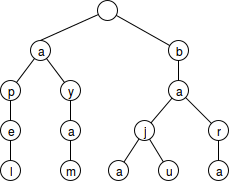
\includegraphics[scale=0.6]{pics/Contoh-StandardTrie}
    \caption{Contoh Standard Trie}
    \label{fig:contoh-standard-trie}
\end{figure}

%-----------------------------------------------------------------------------%
\subsection{Suffix Tree}
%-----------------------------------------------------------------------------% 
\textit{Suffix tree} sering digunakan untuk pencarian sequence yang panjang seperti \textit{genomes} untuk bidang bioinformatik. Pembentukan \textit{suffix tree} mirip seperti \textit{Standard Trie}, namun untuk seluruh \textit{suffix} dalam \textit{string}. Jika diberikan \textit{string} dengan panjang $n$, dibentuk cabang dengan $n(n-1)/2$ \textit{suffix}.  Metode ini banyak dimanfaatkan untuk mempercepat proses pencarian jika diberikan sebuah masukan \textit{query}. Jika terdapat sebuah \textit{pattern} dengan panjang \textit{string} $m$, maka waktu yang dibutuhkan untuk menjalankan proses \textit{pattern matching} adalah $O(dm)$ dengan $d$ adalah ukuran alfabet. Proses pencarian dilakukan dengan menelusuri \textit{path} dari \textit{root} sesuai dengan \textit{sequence query}. Jika seluruh karakter dalam \textit{query} selesai dijalankan, maka proses pencarian berhasil. 

Sebagai contoh \textit{string} 'babaa' menghasilkan \textit{suffix tree} berikut. Jika diberi \textit{query} 'ba' maka akan berhasil terhadap \textit{path} 'babaa' dan 'baa'.
\begin{figure}
    \centering
    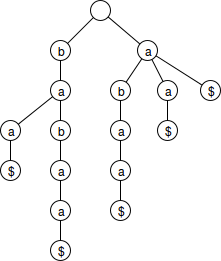
\includegraphics[scale=0.6]{pics/Contoh-SuffixTree}
    \caption{Contoh Suffix Trie}
    \label{fig:contoh-suffix-trie}
\end{figure}

%-----------------------------------------------------------------------------%
%-----------------------------------------------------------------------------%
\section{Semi Supervised}
%-----------------------------------------------------------------------------%
Dalam \textit{machine learning} terdapat dua tipe pendekatan yang umum digunakan yaitu \textit{supervised} dan \textit{unsupervised learning}. Supervised menggunakan data berlabel sebagai data \textit{training} maupun \textit{testing}. Dari kedua data tersebut, dibentuk suatu \textit{classifier} yang dapat memenuhi segala kasus yang mungkin terjadi. Data \textit{testing} digunakan untuk menguji kebaikan \textit{classifier} yang terbentuk. \textit{Unsupervised} menggunakan data yang tidak diberi label sama sekali dan berusaha untuk menemukan pola yang sama untuk suatu kumpulan data tertentu \citep{prakash2014survey}. Pendekatan lain yang merupakan kombinasi antara \textit{supervised} dan \textit{unsupervised learning} adalah \textit{semi supervised learning}. 

\textit{Semi supervised} adalah pendekatan \textit{machine learning} dimana informasi \textit{supervised} data diberikan tidak untuk seluruh data. Sebagian data merupakan data berlabel sementara sebagian lainnya belum memiliki label. Beberapa metode penerapan semi supervised adalah \textit{bootstrapping} (\textit{self training}), \textit{mixture models}, \textit{graph based methods}, \textit{co-training,} dan \textit{multiview learning}.
%(12) MITPress - Semi Supervised Learning

%-----------------------------------------------------------------------------%
\subsection{Bootstrapping}
%-----------------------------------------------------------------------------% 
Model \textit{bootstrapping} merupakan salah satu model \textit{semi supervised learning} yang paling umum digunakan. \textit{Bootstrapping} menggunakan data berlabel berukuran kecil dan data tidak berlabel berukuran jauh lebih besar. Proses anotasi data tidak berlabel dilakukan secara bertahap melalui sejumlah iterasi. Dari data \textit{training} berlabel, dibentuk suatu \textit{classifier} yang kemudian digunakan untuk menganotasi data tidak berlabel. Sejumlah $k$ data baru yang merupakan hasil pelabelan, dimasukkan ke dalam kelompok data berlabel. Proses tersebut dilakukan secara berulang, sehingga semakin lama iterasi jumlah data berlabel akan bertambah. 

Terdapat dua algoritma \textit{bootstrapping} yang pernah digunakan untuk proses \textit{pattern extraction} dan \textit{matching} yaitu \textit{Meta-Bootstrapping} dan \textit{Basilisk} \citep{riloff2003learning}. Keduanya digunakan untuk mengelompokan kata ke dalam suatu kategori semantik jika diberikan korpus teks yang belum dianotasi dan suatu \textit{seed}. \textit{Seed} didefinisikan sebagai korpus kata yang sudah diketahui kategori semantiknya. Secara umum, proses ini akan mencari \textit{pattern} berdasarkan seed yang diberikan. Dari \textit{pattern} yang dihasilkan dan teks yang belum dianotasi, diekstrak entitas baru dan dikelompokan berdasarkan kategori semantiknya. Kata-kata tersebut akan digabungkan ke dalam korpus pasangan kata berelasi.

%-----------------------------------------------------------------------------%
\subsection{Meta Bootstrapping}
%-----------------------------------------------------------------------------% 
Berikut adalah beberapa proses \citep{riloff1999learning} yang dijalankan algoritma \textit{meta bootstrapping} jika diberikan \textit{seed} berukuran kecil yang berasal dari suatu kategori semantik dan korpus yang belum dianotasi.
\begin{enumerate}
  \item Mengekstraksi \textit{pattern} secara otomatis dengan menerapkan syntactic template.
  \item Untuk setiap \textit{pattern} akan diberi bobot berdasarkan jumlah seed yang menghasilkan \textit{pattern}.
  \item Diambil \textit{pattern} terbaik dan seluruh seed lama yang merepresentasikan \textit{pattern} maupun \textit{seed} baru yang berhasil diekstrak disimpan.
  \item Dilakukan pembobotan ulang untuk setiap \textit{pattern} menggunakan \textit{seed} lama dan baru.
\end{enumerate}
Proses diatas dinamakan \textit{mutual bootstrapping} dan setelah proses tersebut selesai, semua entitas baru hasil ekstraksi dievaluasi. Pembobotan entitas baru diberikan berdasarkan jumlah \textit{pattern} yang mengekstrak kata tersebut. Lima kata terbaik diterima dan dimasukkan ke kamus (korpus) kata berelasi untuk selanjutnya diproses ulang.

%-----------------------------------------------------------------------------%
\subsection{Basilisk}
%-----------------------------------------------------------------------------% 
Algoritma \textit{Basilisk} \citep{thelen2002bootstrapping} juga memanfaatkan \textit{pattern} dan \textit{seed} dalam membangun korpus untuk suatu kategori semantik tertentu. Beberapa tahapan yang dijalankan adalah sebagai berikut.
\begin{enumerate}
  \item Secara otomatis membentuk \textit{pattern} dan memberi bobot berdasarkan jumlah seed yang menghasilkan \textit{pattern}. Pattern terbaik dimasukan ke dalam \textit{Pattern Pool}.
  \item Untuk setiap entitas baru yang terekstraksi dari \textit{pattern}, dimasukan ke dalam \textit{Candidate Word Pool}. Pemberian bobot dilakukan berdasarkan jumlah \textit{pattern} yang mengekstraksi dan asosiasi kumulatif kata dengan \textit{seed}.
  \item Sepuluh kata terbaik diambil dan dimasukan ke dalam kamus (korpus) yang kemudian digunakan untuk iterasi selanjutnya. 
\end{enumerate}

Kateogori semantik untuk proses ini bisa lebih dari satu. \textit{Basilisk} memberi bobot berdasarkan informasi kolektif dari kumpulan \textit{pattern} yang mengekstrak kata tersebut. Sementara \textit{Meta-Bootstrapping} hanya mengambil satu \textit{pattern} terbaik dan mengelompokkan seluruh kata yang terekstrak dari \textit{pattern} ke dalam kategori semantik yang sama. Dari hasil penelitian komparatif yang pernah dilakukan \citep{riloff2003learning}, didapatkan \textit{Basilisk} mengungguli performa \textit{Meta-Bootstrapping}. 

%-----------------------------------------------------------------------------%
%-----------------------------------------------------------------------------%
\section{Word Embedding}
%-----------------------------------------------------------------------------%
\textit{Word Embedding} digunakan untuk menentukan similarity antar kata relasi yang dihasilkan dari proses \textit{Pattern Matching}.

%-----------------------------------------------------------------------------%
%-----------------------------------------------------------------------------%
\section{Pointwise Mutual Information}
%-----------------------------------------------------------------------------%
\textit{Pointwise Mutual Information} (PMI) adalah pengukuran nilai asosiasi antar variabel. Dalam bidang \textit{information theory}, PMI dapat dimanfaatkan untuk menghitung asosiasi kemunculan dua buah kata. Jika diberikan dua buah kata $x$ dan $y$, maka nilai PMI kata tersebut dalam suatu dokumen dapat dihitung menggunakan rumus berikut. 
\[ pmi(x;y)=log\frac{p(x,y)}{(x)p(y)}=log\frac{p(x|y)}{p(x)}=log\frac{p(y|x)}{p(y)} \] dengan $p(x)=\frac{f(x)}{N}$
\[ pmi(x;y)=log\frac{f(x)N}{f(x)f(y)} \]
\begin{itemize}
  \item $p(x)$ adalah probabilitas kemunculan kata $x$ dalam korpus
  \item $f(x)$ adalah frekuensi kemunculan kata $x$ dalam korpus
  \item $N$ adalah toatal seluruh kata dalam korpus
\end{itemize}
Pengukuran ini bersifat simetris, sehingga $p(x;y)=p(y;x)$. Nilai PMI dapat merupakan bilangan positif maupun negatif. Jika nilai PMI adalah nol (0), berarti kedua variabel saling \textit{independent}.

%-----------------------------------------------------------------------------%
\subsection{Skip PMI}
%-----------------------------------------------------------------------------% 
PMI umumnya hanya menggunakan model \textit{bigram} atau \textit{trigram}. Model ini hanya melihat hubungan kata yang berdampingan. Sebagai contoh ingin diketahui PMI untuk \textit{bigram} 'hong kong', 'sepak bola', dan 'amerika serikat'. Pada penelitian ini dilakukan modifikasi yaitu membuat model \textit{skip-gram} PMI. Kita menghitung nilai PMI antar dua kata yang dipisahkan dengan $n$ diantaranya. 

%-----------------------------------------------------------------------------%
%-----------------------------------------------------------------------------%
\section{Evaluasi}
%-----------------------------------------------------------------------------%
Evaluasi dilakukan untuk mengetahui kebaikan hasil penelitian. Evaluasi dapat dilakukan dengan mengukur akurasi data yang dihasilkan. Akurasi adalah nilai perbandingan antara jumlah data yang benar dengan jumlah seluruh data (Manning). 
\[ akurasi=\frac{jumlah\,\,data\,\,benar}{jumlah\,\,seluruh\,\,data} \]
Selain menghitung akurasi, proses evaluasi juga menghitung nilai-nilai lainnya. Berikut ada beberapa metode dan teknik evaluasi lain yang digunakan dalam penelitian.

%-----------------------------------------------------------------------------%
\subsection{Sampling}
%-----------------------------------------------------------------------------% 
Terdapat dua kategori utama dalam \textit{sampling} yaitu \textit{probability} dan \textit{non-probability sampling}. Perbedaan utama keduanya adalah pada \textit{probability sampling}, diambil data secara acak (\textit{random}). Dalam \textit{probability sampling}, terdapat beberapa metode yang dapat digunakan seperti \textit{simple random sampling}, \textit{systematic sampling}, \textit{stratified random sampling}, dan \textit{cluster sampling}.
\begin{itemize}
  \item \textit{Simple random sampling} perlu mengetahui seluruh data yang ada dan dari data tersebut dipilih secara acak. Hal ini membuat seluruh data memiliki nilai probabilitas terpilih yang sama. 
  \item \textit{Systematic sampling} memilih setiap data ke-n untuk dijadikan \textit{sample}. 
  \item \textit{Stratified random sampling} akan mengelompokan data ke dalam kategori berdasarkan karakteristik tertentu (strata), kemudian data diambil secara acak dari kategori yang ada. Hal ini menyebabkan hasil lebih representatif. 
  \item \textit{Cluster} sampling mirip seperti \textit{stratified sampling} namun dilakukan jika data kelompok yang ingin di-\textit{sampling} sulit berada di lokasi yang terpisah jauh.
\end{itemize}
Proses \textit{sampling} bermanfaat untuk merepresentasikan data tanpa perlu mengevaluasi seluruh data yang ada. Jika jumlah data yang ingin dievaluasi berukuran besar, proses \textit{sampling} mempercepat pengukuran. Jumlah data yang direpresentasikan oleh satu sample berdasarkan jumlah data asli. Sebagai contoh jika total data adalah 1000 dan jumlah data sample adalah 50, maka satu data \textit{sample} merepresentasikan 20 data asli.
%(Sumber: https://ecduganda.files.wordpress.com/2014/08/how-to-choose-sampling-techniques-for-evaluations.pdf)
%(http://optimierung.mathematik.uni-kl.de/mamaeusch/veroeffentlichungen/ver_texte/sampling_en.pdf)

%-----------------------------------------------------------------------------%
\subsection{Precision dan Recall}
%-----------------------------------------------------------------------------% 
Teknik yang umum digunakan untuk mengevaluasi suatu ekstraksi adalah \textit{precision} dan \textit{recall}. \textit{Precision} adalah nilai yang menyatakan jumlah dokumen benar dan berhasil diambil dibandingkan dengan seluruh jumlah dokumen yang terambil. \textit{Recall} adalah nilai yang menyatakan jumlah dokumen benar dan berhasil diambil dibandingkan dengan jumlah seluruh dokumen yang benar. Semakin banyak dokumen yang diambil maka nilai \textit{recall} akan meningkat sementara nilai \textit{precision} cenderung menurun. 

%-----------------------------------------------------------------------------%
\subsection{Kappa}
%-----------------------------------------------------------------------------%  
Nilai kappa ($\kappa$) merepresentasikan tingkat persetujuan antar anotator. Kappa digunakan pada penelitian yang menggunakan bantuan anotator untuk memberi penilaian secara manual. Peniliaian didapatkan menggunakan rumus berikut.
\[ \kappa=\frac{P(A)-P(E)}{1-P(E)} \]
\begin{itemize}
  \item $P(A)$ adalah proporsi penilaian yang setuju (\textit{agreement})
  \item $P(E)$ adalah proporsi penilaian yang kebetulan
\end{itemize}
\cite{landis1977measurement} mendefiniskan tingkat persetujuan berdasarkan nilai Kappa yang diperoleh. 
\begin{table}
  \centering
    \caption{Skala pengukuran Kappa}
    \label{table:skalaKappa}
    \begin{tabular}{|c|c|}
      \hline
      Statistik Kappa & Tingkat persetujuan \\ \hline
      < 0.00 & \textit{Poor} \\ \hline
      0.00 - 0.20 & \textit{Slight} \\ \hline
      0.21 - 0.40 & \textit{Fair} \\ \hline
      0.41 - 0.60 & \textit{Moderate} \\ \hline
      0.61 - 0.80 & \textit{Substantial} \\ \hline
      0.81 - 1.00 & \textit{Almost Perfect} \\ \hline
    \end{tabular}
\end{table}

Beberapa variasi perhitungan untuk Kappa adalah Cohen's Kappa dan Fleiss' Kappa. Cohen's Kappa digunakan untuk mengukur tingkat persetujuan antar dua anotator. Jika diberikan data dengan $n$ label dan $m_ij$ merepresentasikan jumlah data yang diberi label $i$ oleh anotator pertama dan label $j$ oleh anotator kedua, maka proses perhitungan $P(A)$ dan $P(E)$ untuk Cohen's Kappa adalah sebagai berikut.
\[ P(A)=\frac{\sum_{k=1}^{n} m_kk}{total\,\,data} \]
\[ P(E)=\frac{\sum_{k=1}^{n} ( \sum_{j=1}^{n} m_kj . \sum_{i=1}^{n} m_ik ) }{total\,\,data} \]

Fleiss' Kappa mengukur tingkat persetujuan antar sekelompok anotator berjumlah lebih dari dua. Jika diberikan $N$ data dengan $n$ anotator dimana setiap data diantosi ke dalam salah satu dari $k$ kategori dan $n_ij$ merepresentasikan total anotator yang memberi data $i$ ke label $j$, proses perhitungan $P(A)$ dan $P(E)$ untuk Fleiss' Kappa adalah sebagai berikut.
\[ P(A)=\frac{1}{N}\sum_{i=1}^{N}P_i \:\:\:\:\:dengan\:\:\:\:\: P_i=\frac{1}{n(n-1)}[(\sum_{j=1}^{k}n^2_ij)-(n)] \]


%-----------------------------------------------------------------------------%
\subsection{Spearman's Rho}
%-----------------------------------------------------------------------------% 
\textit{Spearman's rank correlation coefficient} adalah nilai koefisien korelasi antar \textit{ranking} dua parameter. Nilai \textit{Spearman correlation} sama dengan nilai \textit{Pearson correlation} antar dua paramter yang telah di-\textit{ranking}. \textit{Pearson correlation}  menggambarkan nilai linear antara dua parameter. \textit{Spearman correlation} berkisar antara $-1$ hingga $+1$.

Spearman's rho adalah nilai Pearson Correlation Coefficient antar dua variabel yang telah di-\textit{ranking}. Untuk mendapatkan nilai koefisien ($r_s$), menggunakan rumus berikut.
\[ r_s = \rho_{rg_X,rg_Y} = \frac{cov(rg_X,rg_Y)}{\sigma_{rg_X}\sigma_{rg_Y}} \]
\begin{itemize}
  \item $\rho$ adalah \textit{Pearson correlation coefficent} yang diaplikasikan pada variabel \textit{ranking}
  \item $cov(rg_X,rg_Y)$ adalah nilai \textit{covariance} antar variabel \textit{ranking}
  \item $\sigma_{rg_X}$ dan $\sigma_{rg_Y}$ adalah nilai standard deviasi variabel \textit{ranking}
\end{itemize}
Jika seluruh \textit{ranking} berbeda, proses komputasi dapat dilakukan menggunakan rumus berikut.
\[ r_s = 1-\frac{6 \Sigma d_i^2}{n(n^2-1)} \]
\begin{itemize}
  \item $d_i = rg(X_i)-rg(Y_i)$ adalah selisih antara dua \textit{ranking}
  \item $n$ adalah jumlah observasi
\end{itemize}

%%-----------------------------------------------------------------------------%
\chapter{\babTiga}
%-----------------------------------------------------------------------------%

%-----------------------------------------------------------------------------%
\section{NPACI Rocks}
%-----------------------------------------------------------------------------%

%-----------------------------------------------------------------------------%
\subsection{XZXX}
%-----------------------------------------------------------------------------%
Ini dapat dilihat di Gambar \ref{fig:alurkickstart} \citep{paper.jackson}. 

\begin{figure}
	\centering
	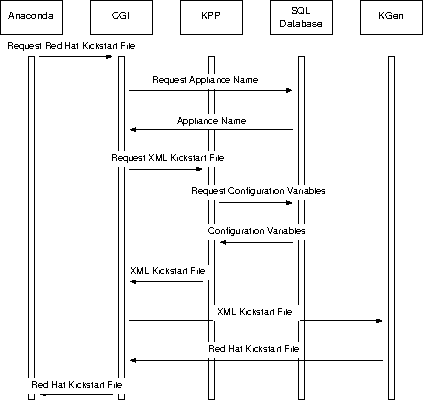
\includegraphics[width=0.8\textwidth,height=0.7\textwidth]
		{pics/alurkickstart.pdf}
	\caption{Alur Perjalanan \f{Kickstart}}
	\label{fig:alurkickstart}
\end{figure}
\begin{center}
{\small Sumber gambar: \citep{paper.jackson}}
\end{center}

Kata-kata dalam gambarnya bisa di hover, magic!!

%-----------------------------------------------------------------------------%
\subsection{Rocks Rolls}
%-----------------------------------------------------------------------------%
Untuk contoh konten Rolls dapat dilihat pada gambar \ref{fig:contohisiroll}. Pada contoh tersebut, \f{package} yang mengandung konfigurasi \f{graph} adalah berkas \co{roll-sge-kickstart-3.2.0-0.noarch.rpm} \citep{paper.jackson}. 


\begin{figure}
	\centering
	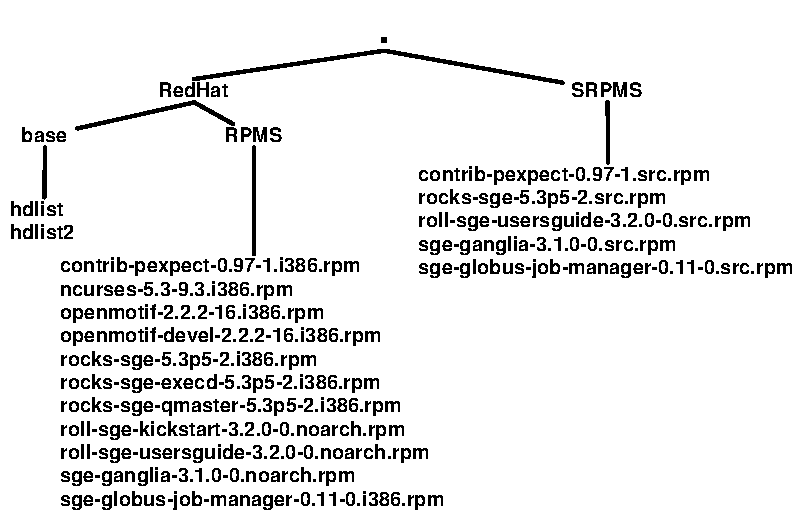
\includegraphics[width=0.9\textwidth,height=0.6\textwidth]
		{pics/rollexample.pdf}
	\caption{Contoh konten yang berada dalam \f{Rolls}}
	\label{fig:contohisiroll}
\end{figure}
\begin{center}
{\small Sumber gambar: \citep{paper.jackson}}
\end{center}

COde-like words : \code{FIRSTFIT} atau \code{BESTFIT} \citep{paper.jackson}. 

%-----------------------------------------------------------------------------%
\section{Mengubah Tampilan Teks}
%-----------------------------------------------------------------------------%
Beberapa perintah yang dapat digunakan untuk mengubah tampilan adalah: 
\begin{itemize}
	\item \bslash f \\
		Merupakan alias untuk perintah \bslash textit, contoh 
		\f{contoh hasil tulisan}.
	\item \bslash bi \\
		\bi{Contoh hasil tulisan}.
	\item \bslash bo \\
		\bo{Contoh hasil tulisan}.
	\item \bslash code \\ 
		\code{Contoh hasil tulisan}.
\end{itemize}


%-----------------------------------------------------------------------------%
\section{Memberikan Catatan}
%-----------------------------------------------------------------------------%
Ada dua perintah untuk memberikan catatan penulisan dalam dokumen yang Anda 
kerjakan, yaitu: 
\begin{itemize}
	\item \bslash todo \\
		Contoh: \\ \todo{Contoh bentuk todo.}
	\item \bslash todoCite \\ 
		Contoh: \todoCite
\end{itemize}


%-----------------------------------------------------------------------------%
\section{Menambah Isi Daftar Isi}
%-----------------------------------------------------------------------------%
Terkadang ada kebutuhan untuk memasukan kata-kata tertentu kedalam Daftar Isi. 
Perintah \bslash addChapter dapat digunakan untuk judul bab dalam Daftar isi. 
Contohnya dapat dilihat pada berkas thesis.tex.
%%-----------------------------------------------------------------------------%
\chapter{\babEmpat}
%-----------------------------------------------------------------------------%
%-----------------------------------------------------------------------------%
\section{Membuat Tabel}
%-----------------------------------------------------------------------------%
Seperti pada gambar, tabel juga dapat diberi label dan caption. 
Caption pada tabel terletak pada bagian atas tabel. 
Contoh tabel sederhana dapat dilihat pada \tab~\ref{tab:tab1}.

\begin{table}
	\centering
	\caption{Contoh Tabel}
	\label{tab:tab1}
	\begin{tabular}{| l | c r |}
		\hline
		& kol 1 & kol 2 \\ 
		\hline
		baris 1 & 1 & 2 \\
		baris 2 & 3 & 4 \\
		baris 3 & 5 & 6 \\
		jumlah  & 9 & 12 \\
		\hline
	\end{tabular}
\end{table}

Ada jenis tabel lain yang dapat dibuat dengan \latex~berikut 
beberapa diantaranya. 
Contoh-contoh ini bersumber dari 
\url{http://en.wikibooks.org/wiki/LaTeX/Tables}

\begin{table}
	\centering
	\caption{An Example of Rows Spanning Multiple Columns}
	\label{row.spanning}
	\begin{tabular}{|l|l|*{6}{c|}}
  		\hline % create horizontal line
  		No & Name & \multicolumn{3}{|c|}{Week 1} & \multicolumn{3}{|c|}{Week 2} \\
  		\cline{3-8} % create line from 3rd column till 8th column
  		& & A & B & C & A & B & C\\
  		\hline
  		1 & Lala & 1 & 2 & 3 & 4 & 5 & 6\\
  		2 & Lili & 1 & 2 & 3 & 4 & 5 & 6\\
  		3 & Lulu & 1 & 2 & 3 & 4 & 5 & 6\\
  		\hline
	\end{tabular}
\end{table}

\begin{table}
	\centering
	\caption{An Example of Columns Spanning Multiple Rows}
	\label{column.spanning}
	\begin{tabular}{|l|c|l|}
		\hline
		Percobaan & Iterasi & Waktu \\
		\hline
		Pertama & 1 & 0.1 sec \\ \hline
		\multirow{2}{*}{Kedua} & 1 & 0.1 sec \\
 		& 3 & 0.15 sec \\ 
 		\hline
		\multirow{3}{*}{Ketiga} & 1 & 0.09 sec \\
 		& 2 & 0.16 sec \\
 		& 3 & 0.21 sec \\ 
 		\hline
	\end{tabular}
\end{table}

\begin{table}
	\centering
	\caption{An Example of Spanning in Both Directions Simultaneously}
	\label{mix.spanning}
	\begin{tabular}{cc|c|c|c|c|}
		\cline{3-6}
		& & \multicolumn{4}{|c|}{Title} \\ \cline{3-6}
		& & A & B & C & D \\ \hline
		\multicolumn{1}{|c|}{\multirow{2}{*}{Type}} &
		\multicolumn{1}{|c|}{X} & 1 & 2 & 3 & 4\\ \cline{2-6}
		\multicolumn{1}{|c|}{}                        &
		\multicolumn{1}{|c|}{Y} & 0.5 & 1.0 & 1.5 & 2.0\\ \cline{1-6}
		\multicolumn{1}{|c|}{\multirow{2}{*}{Resource}} &
		\multicolumn{1}{|c|}{I} & 10 & 20 & 30 & 40\\ \cline{2-6}
		\multicolumn{1}{|c|}{}                        &
		\multicolumn{1}{|c|}{J} & 5 & 10 & 15 & 20\\ \cline{1-6}
	\end{tabular}
\end{table}

%-----------------------------------------------------------------------------%
\section{thesis.tex}
%-----------------------------------------------------------------------------%
Berkas ini berisi seluruh berkas Latex yang dibaca, jadi bisa dikatakan sebagai 
berkas utama. Dari berkas ini kita dapat mengatur bab apa saja yang ingin 
kita tampilkan dalam dokumen.


%-----------------------------------------------------------------------------%
\section{laporan\_setting.tex}
%-----------------------------------------------------------------------------%
Berkas ini berguna untuk mempermudah pembuatan beberapa template standar. 
Anda diminta untuk menuliskan judul laporan, nama, npm, dan hal-hal lain yang 
dibutuhkan untuk pembuatan template. 


%-----------------------------------------------------------------------------%
\section{istilah.tex}
%-----------------------------------------------------------------------------%
Berkas istilah digunakan untuk mencatat istilah-istilah yang digunakan. 
Fungsinya hanya untuk memudahkan penulisan.
Pada beberapa kasus, ada kata-kata yang harus selalu muncul dengan tercetak 
miring atau tercetak tebal. 
Dengan menjadikan kata-kata tersebut sebagai sebuah perintah \latex~tentu akan 
mempercepat dan mempermudah pengerjaan laporan. 


%-----------------------------------------------------------------------------%
\section{hype.indonesia.tex}
%-----------------------------------------------------------------------------%
Berkas ini berisi cara pemenggalan beberapa kata dalam bahasa Indonesia. 
\latex~memiliki algoritma untuk memenggal kata-kata sendiri, namun untuk 
beberapa kasus algoritma ini memenggal dengan cara yang salah. 
Untuk memperbaiki pemenggalan yang salah inilah cara pemenggalan yang benar 
ditulis dalam berkas hype.indonesia.tex.
%%-----------------------------------------------------------------------------%
\chapter{\babLima}
%-----------------------------------------------------------------------------%

%-----------------------------------------------------------------------------%
\section{Implementasi \f{Cluster}}
%-----------------------------------------------------------------------------%

%-----------------------------------------------------------------------------%
\subsection{Instalasi \f{Frontend}}
%-----------------------------------------------------------------------------%
Tabel model lain, ditunjukkan pada tabel \ref{tab:infohasti}. 
\begin{table}
	\centering
	\caption{Informasi \f{cluster} X}
	\newcolumntype{g}{>{\columncolor{headertbl}}c}
	\label{tab:infohasti}
	\begin{tabular}{|g|c|}
	\hline Host Name & X\\
	\hline Cluster Name & X\\
	\hline Certificate Organization & UI\\
	\hline Certificate Locality & Depok\\
	\hline Certificate State & West Java\\
	\hline Certificate Country & ID\\
	\hline Contact & X\\
	\hline URL & http://grid.ui.ac.id\\
	\hline
	\end{tabular}
\end{table}

Ada pagebreak disini.
%supaya rapih
\pagebreak

Another type of table
\begin{table}
	\centering
	\caption{Perbandingan Partisi \f{default} dan manual}
	\newcolumntype{g}{>{\columncolor{headertbl}}c}
	\label{tab:partdisk}
	\begin{tabular}{|g|c|c|}
	\rowcolor{headertbl}
	\hline & Partisi default & Partisi manual yang dilakukan\\
	\hline / & 16 GB & 30 GB\\
	\hline /var & 4 GB & 18 GB\\
	\hline swap & 1 GB & 2 GB\\
	\hline /export & 55 GB & 26 GB\\
	\hline
	\end{tabular}
\end{table}

Program menghasilkan keluaran seperti pada kode \ref{lst:raidready}. 

\begin{minipage}{\linewidth}
\begin{lstlisting}[caption={Keluaran output},label={lst:raidready}]
[root@nas-0-0 ~]# cat /proc/mdstat 
Personalities : [raid1] 
md0 : active raid1 sda4[0] sdb2[1]
      1917672312 blocks super 1.2 [2/2] [UU]
      
unused devices: <none>
[root@nas-0-0 ~]# mdadm --detail /dev/md0 
/dev/md0:
        Version : 1.2
  Creation Time : Fri May  3 15:38:52 2013
     Raid Level : raid1
     Array Size : 1917672312 (1828.83 GiB 1963.70 GB)
  Used Dev Size : 1917672312 (1828.83 GiB 1963.70 GB)
   Raid Devices : 2
  Total Devices : 2
    Persistence : Superblock is persistent

    Update Time : Tue May 28 11:27:49 2013
          State : clean 
 Active Devices : 2
Working Devices : 2
 Failed Devices : 0
  Spare Devices : 0

           Name : nas-0-0.local:0  (local to host nas-0-0.local)
           UUID : 0754726d:3dfbd4b9:42b0f587:68631556
         Events : 28

    Number   Major   Minor   RaidDevice State
       0       8        4        0      active sync   /dev/sda4
       1       8       18        1      active sync   /dev/sdb2
\end{lstlisting}
\end{minipage}

%-----------------------------------------------------------------------------%
\subsection{Konfigurasi}\label{cha:confcluster}
%-----------------------------------------------------------------------------%
Contoh verbatim dalam itemize : 
\begin{itemize}
\item \bo{Bold ini}\\
dijalankan perintah berikut : 
\begin{Verbatim}[frame=single]
# javac Ganteng.java
# java Ganteng
\end{Verbatim}
\paragraph{}
Perilaku sistem 
\begin{Verbatim}[frame=single]
# hai
# enable
# cd /export/rocks/install/
# create distro
# sh sesuatu.sh
# reboot
\end{Verbatim}
\paragraph{}

\item \bo{Menambahkan \f{package} pada \f{compute node}}\\
Langkah yang dilakukan adalah sebagai berikut : 
	\begin{enumerate}
	\item Masuk ke dalam direktori \co{/procfs/}
	\item Membuat/Mengubah berkas \co{xx.xml}. Jika tidak terdapat berkas tersebut, dapat disalin dari \co{skeleton.xml}.
	\item Menambahkan \f{package} yang ingin dipasang pada \f{compute node} diantara \f{tag} \co{<package>} seperti berikut : \co{<package>[package yang akan dipasang]</package>}.
	\item Menjalankan perintah berikut termasuk perintah untuk melakukan instalasi ulang seluruh \f{compute node}: 
	\begin{Verbatim}[frame=single]
# cd /export/somedir
# create
# run host
	\end{Verbatim}
	\end{enumerate}
	\paragraph{}
\end{itemize}
%-----------------------------------------------------------------------------%
\subsubsection{semakin ke dalam}
%-----------------------------------------------------------------------------%
\begin{minipage}{\linewidth}
\begin{lstlisting}[caption={Keluaran mentah untuk detail \f{job}}, label={lst:outqstatf},style=L]
[ardhi@xx ~]$ qstat -f 138
Job Id: 138.xx
    Job_Name = cur-1000-1np
    Job_Owner = ardhi@xx
    resources_used.cput = 27:21:35
    resources_used.mem = 86060kb
    resources_used.vmem = 170440kb
    resources_used.walltime = 27:24:50
    job_state = R
    queue = default
    server = hastinapura.grid.ui.ac.id
    Checkpoint = u
    ctime = Fri May 31 10:27:37 2013
    Error_Path = xx:/home/ardhi/xx/curcumin-1000/cur-1000-1np.e138
    exec_host = compute-0-5/0
    exec_port = 15003
    Hold_Types = n
    Join_Path = n
    Keep_Files = n
    Mail_Points = e
    Mail_Users = ardhi.putra@ui.ac.id
    mtime = Fri May 31 10:27:47 2013
    Output_Path = xx:/home/ardhi/xx/curcumin-1000/cur-1000-1np.o138
    Priority = 0
    qtime = Fri May 31 10:27:37 2013
    Rerunable = True
    Resource_List.nodes = 1:ppn=1
    session_id = 5768
    etime = Fri May 31 10:27:37 2013
    submit_args = cur-1000-1np.pbs
    start_time = Fri May 31 10:27:47 2013
    submit_host = xx
    init_work_dir = /home/ardhi/xx/curcumin-1000   
\end{lstlisting}
\end{minipage}

%-----------------------------------------------------------------------------%
\section{Pengujian} %lebih ke gimana cara ujinya
%-----------------------------------------------------------------------------%

%-----------------------------------------------------------------------------%
\subsection{Kasus Uji}
%-----------------------------------------------------------------------------%
Berwarna!
\begin{lstlisting}[caption=Potongan skrip submisi \f{job} melalui torqace,label={lst:grotorqace},style=shell]
# Go To working directory
cd $PBS_O_WORKDIR

#openMPI prerequisite
. /opt/torque/etc/openmpi-setup.sh

mpirun -np 5 -machinefile $PBS_NODEFILE mdrun -v -s \ 
	curcum400ps.tpr -o md_prod_curcum400_5np.trr -c lox_pr.gro
...
\end{lstlisting}
%-----------------------------------------------------------------------------%
\subsection{Kasus Uji}
%-----------------------------------------------------------------------------%
Contoh skrip yang dimasukkan pada \f{form} yang disediakan dapat dilihat pada kode \ref{lst:makebzip}.
\begin{lstlisting}[caption={Potongan \co{Makefile} \f{project}}, label={lst:makebzip},style=shell]
# Make file for MPI
SHELL=/bin/sh

# Compiler to use
# You may need to change CC to something like CC=mpiCC
# openmpi : mpiCC
# mpich2  : /opt/mpich2/gnu/bin/mpicxx
CC=mpiCC
...
...
\end{lstlisting}
%%-----------------------------------------------------------------------------%
\chapter{\babEnam}
%-----------------------------------------------------------------------------%

%-----------------------------------------------------------------------------%
\section{Hasil Pengujian}
%-----------------------------------------------------------------------------%
%-----------------------------------------------------------------------------%
\subsection{Hasil Pengujian Kasus Uji 1}
%-----------------------------------------------------------------------------%
Tabel lain. Hasil tersebut dapat dilihat pada tabel \ref{tab:hasilgrrd}.
\begin{table}
	\centering
	\caption{Hasil pengujian menggunakan gromacs}
	\label{tab:hasilgrrd}
	\begin{tabular}{|c|l|*{3}{c|}}
		\rowcolor{headertbl}
  		\hline % create horizontal line
  		No & \f{Timestep} & \multicolumn{3}{|>{\columncolor{headertbl}}c|}{Waktu eksekusi berdasar jumlah prosesor} \\
		\hhline{|>{\arrayrulecolor{headertbl}}*{2}{-}>{\arrayrulecolor{black}}*{3}{|-|}}
  		\rowcolor{headertbl} & & 1 & 2 & 5 \\
  		\hline 1 & 200ps & 20h:27m:16s & 12h:59m:04s & 5h:07m:03s \\
  		\hline 2 & 400ps & 1d:22h:40m:03s & 1d:02h:08m:47s & 10h:09m:39s \\
  		\hline 3 & 600ps & 2d:23h:29m:21s & 1d:14h:52m:52s & 15h:25m:22s \\
  		\hline 4 & 800ps & 4d:02h:05m:57s & 2d:03h:30m:07s & 20h:29m:38s \\
  		\hline 5 & 1000ps & 5d:03h:29m:12s & 2d:16h:32m:22s & 1d:01h:34m:38s \\
  		\hline
	\end{tabular}
\end{table}
%-----------------------------------------------------------------------------%
\section{Evaluasi Hasil Kasus Uji}
%-----------------------------------------------------------------------------%
%-----------------------------------------------------------------------------%
\subsection{Evaluasi Kasus Uji 1}
%-----------------------------------------------------------------------------%
Tabel \ref{tab:hasilgrrd} menunjukkan hasil uji coba pada penelitian ini.  Gambar \ref{fig:grafgro5} menunjukkan perbandingan waktu eksekusi pada aplikasi x dengan jumlah prosesor sebanyak 5 buah.

\begin{figure}
	\centering
	\includegraphics[width=1\textwidth]
		{pics/5np-gromacs-chart.pdf}
	\caption{Perbandingan waktu eksekusi x untuk 5 prosesor}
	\label{fig:grafgro5}
\end{figure}
\paragraph{}
%%-----------------------------------------------------------------------------%
\chapter{\babTujuh}
%-----------------------------------------------------------------------------%
Pada bab terakhir ini, 
%---------------------------------------------------------------
\section{Kesimpulan}
%---------------------------------------------------------------

%---------------------------------------------------------------
\section{Saran}
%---------------------------------------------------------------


%\printbibliography
%
% Daftar Pustaka
%\include{pustaka}
%biblama (bukan biblatex)
\bibliography{bib}{}
%\bibliography{references}{}
%biblama (bukan biblatex)
\bibliographystyle{apalikerd}
%\bibliographystyle{ieeetr} 

%
% Lampiran 
%
%\begin{appendix}
%	%
% @author  Andreas Febrian
% @version 1.00 
% 
% Hanya sebuah pembatas bertuliskan LAMPIRAN ditengah halaman. 
% 

\begin{titlepage}
	\centering 
	\vspace*{6cm}
	\noindent \Huge{LAMPIRAN}
	\addChapter{LAMPIRAN}
\end{titlepage} 
%	\setcounter{page}{2}
%	%-----------------------------------------------------------------------------%
\addChapter{Lampiran 1 : Pattern Buatan Manual}
\chapter*{Lampiran 1 : Pattern Buatan Manual}
%-----------------------------------------------------------------------------%
Berikut adalah daftar \textit{pattern} yang dibentuk secara manual oleh anotator.
\begin{itemize}
  \item <hypernym> adalah kumpulan dari <hyponym>
  \item <hypernym> antara lain adalah <hyponym>, <hyponym>, dan <hyponym>
  \item <hypernym> dapat dibedakan menjadi <hyponym>
  \item <hypernym> lainnya, seperti <hyponym> dan <hyponym>
  \item <hypernym> seperti <hyponym>
  \item <hypernym> terdiri dari <hyponym>, <hyponym>, dan <hyponym>
  \item <hypernym> terdiri dari beberapa bagian, seperti <hyponym>, <hyponym>, dan <hyponym>
  \item <hypernym> terutama <hyponym> yang
  \item <hypernym>, khususnya <hyponym>, adalah
  \item <hypernym>, misalnya <hyponym>
  \item <hypernym>, misalnya <hyponym> dan <hyponym>
  \item <hypernym>, terutama <hyponym>, adalah
  \item <hyponym> adalah <hypernym>
  \item <hyponym> adalah <hypernym> dari
  \item <hyponym> adalah <hypernym> dengan
  \item <hyponym> adalah <hypernym> yang berhubungan dekat dengan <hyponym>
  \item <hyponym> adalah <hypernym> yang bersifat
  \item <hyponym> adalah bagian dari <hypernym> yang
  \item <hyponym> adalah salah satu <hypernym>
  \item <hyponym> adalah sebuah <hypernym> yang
  \item <hyponym> adalah sejenis <hypernym> dengan
  \item <hyponym> adalah suatu <hypernym>
  \item <hyponym> atau <hyponym> adalah suatu jenis <hypernym> yang
  \item <hyponym> berarti <hypernym>
  \item <hyponym> dan <hyponym> dianggap sebagai <hypernym>
  \item <hyponym> dan <hyponym> merupakan <hypernym> yang
  \item <hyponym> dan berbagai <hyponym> lainnya adalah <hypernym> yang
  \item <hyponym> dan sejumlah <hyponym> lainnya termasuk ke dalam kategori <hypernym>
  \item <hyponym> dapat digolongkan ke dalam <hypernym>
  \item <hyponym> dapat dimasukkan ke dalam kategori <hypernym> dan <hypernym>
  \item <hyponym> dianggap sebagai <hypernym> karena
  \item <hyponym> dikenal juga sebagai <hypernym>
  \item <hyponym> disebut sebagai <hypernym> yang
  \item <hyponym> ialah <hypernym>
  \item <hyponym> menjadi <hypernym> apabila
  \item <hyponym> menjadi <hypernym> yang
  \item <hyponym> menjadi salah satu bagian dari <hypernym> karena
  \item <hyponym> merujuk pada <hypernym>
  \item <hyponym> merujuk pada <hypernym> yang
  \item <hyponym> merupakan <hypernym>
  \item <hyponym> merupakan <hypernym> yang
  \item <hyponym> merupakan suatu <hypernym> yang
  \item <hyponym> secara khusus menjadi sebutan bagi <hypernym> yang
  \item <hyponym> termasuk <hypernym> yang
  \item <hyponym> termasuk ke dalam <hypernym> yang
  \item <hyponym> termasuk ke dalam kategori <hypernym>
  \item <hyponym> termasuk ke dalam salah satu <hypernym> yang
  \item <hyponym> tersebut merupakan <hypernym>
  \item Beberapa <hypernym> seperti <hyponym>
  \item Beberapa contoh <hypernym> lainnya adalah <hyponym>
  \item Beberapa jenis dari <hypernym> adalah <hyponym> dan <hyponym>
  \item Berbagai <hypernym> seperti <hyponym>
  \item Contoh dari <hypernym> adalah <hyponym>
  \item Contoh dari <hypernym>, yaitu <hyponym>, <hyponym>, dan <hyponym>
  \item Istilah umum dari <hyponym> adalah <hypernym>
  \item Jenis <hypernym> yang paling banyak dikenal adalah <hyponym>
  \item Jenis-jenis <hypernym> antara lain <hyponym> dan <hyponym>
  \item Salah satu <hypernym> adalah <hyponym>
  \item Salah satu <hypernym> yang mirip dengan <hyponym> adalah <hyponym>
  \item Salah satu contoh dari <hypernym> adalah <hyponym>
  \item Sebagai salah satu <hypernym>, <hyponym>
  \item Sebagai sebuah <hypernym>, <hyponym> merupakan
  \item Secara umum, <hyponym> merupakan <hypernym> yang dapat
  \item Selain <hyponym>, <hyponym> juga menjadi <hypernym> yang
  \item Terdapat banyak <hypernym>, seperti <hyponym>
  \item Terdapat beberapa contoh <hypernnym>, di antaranya <hyponym>, <hyponym>, dan <hyponym>
  \item Walaupun <hyponym> adalah <hypernym>, tetapi 
\end{itemize}

%-----------------------------------------------------------------------------%
\addChapter{Lampiran 2 : Panduan Pembuatan dan Anotasi Pattern}
% \chapter*{Lampiran 2 : Panduan Pembuatan danaa Anotasi Pattern}
%-----------------------------------------------------------------------------%
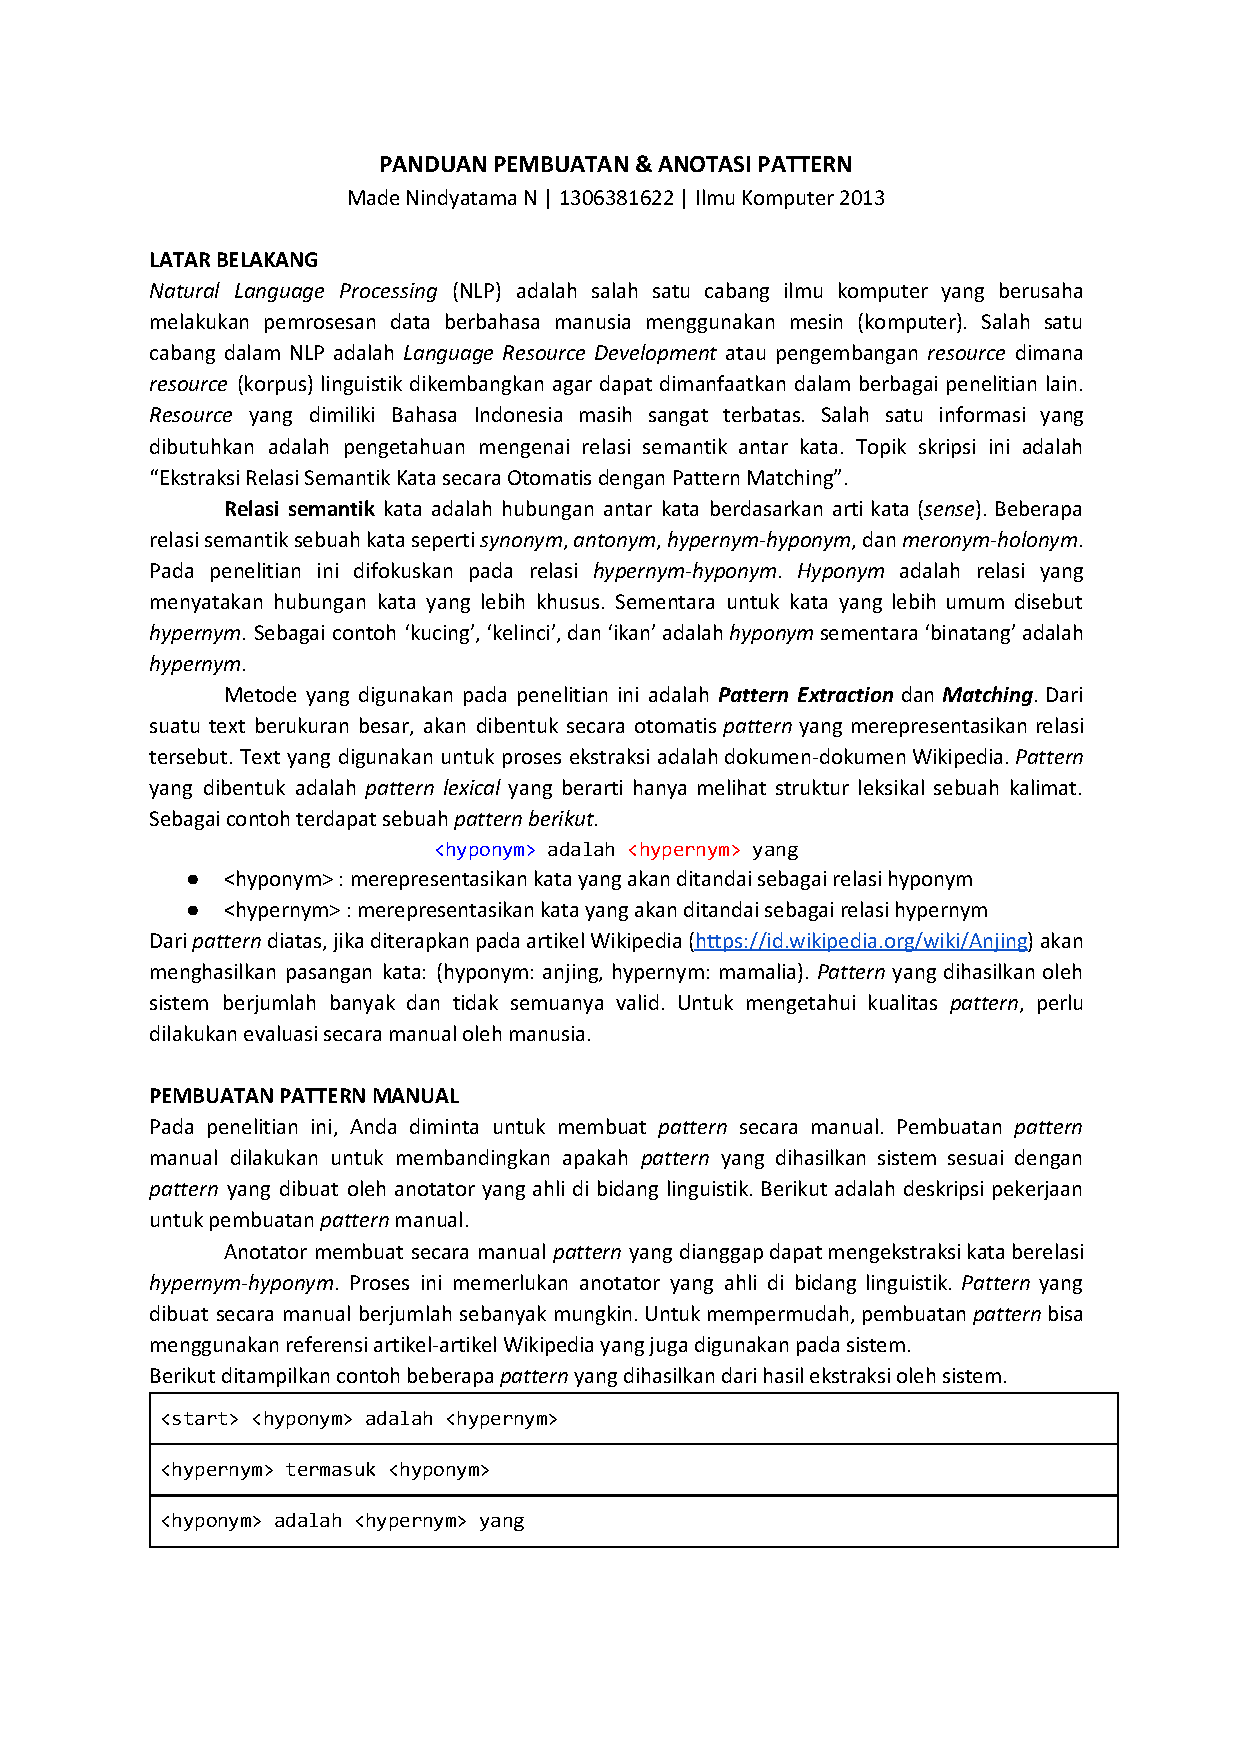
\includepdf[pages={1}]{PanduanPembuatanAnotasiPattern.pdf}
\includepdf[pages={2}]{PanduanPembuatanAnotasiPattern.pdf}

%-----------------------------------------------------------------------------%
\addChapter{Lampiran 3 : Panduan Anotasi Pair}
%-----------------------------------------------------------------------------%
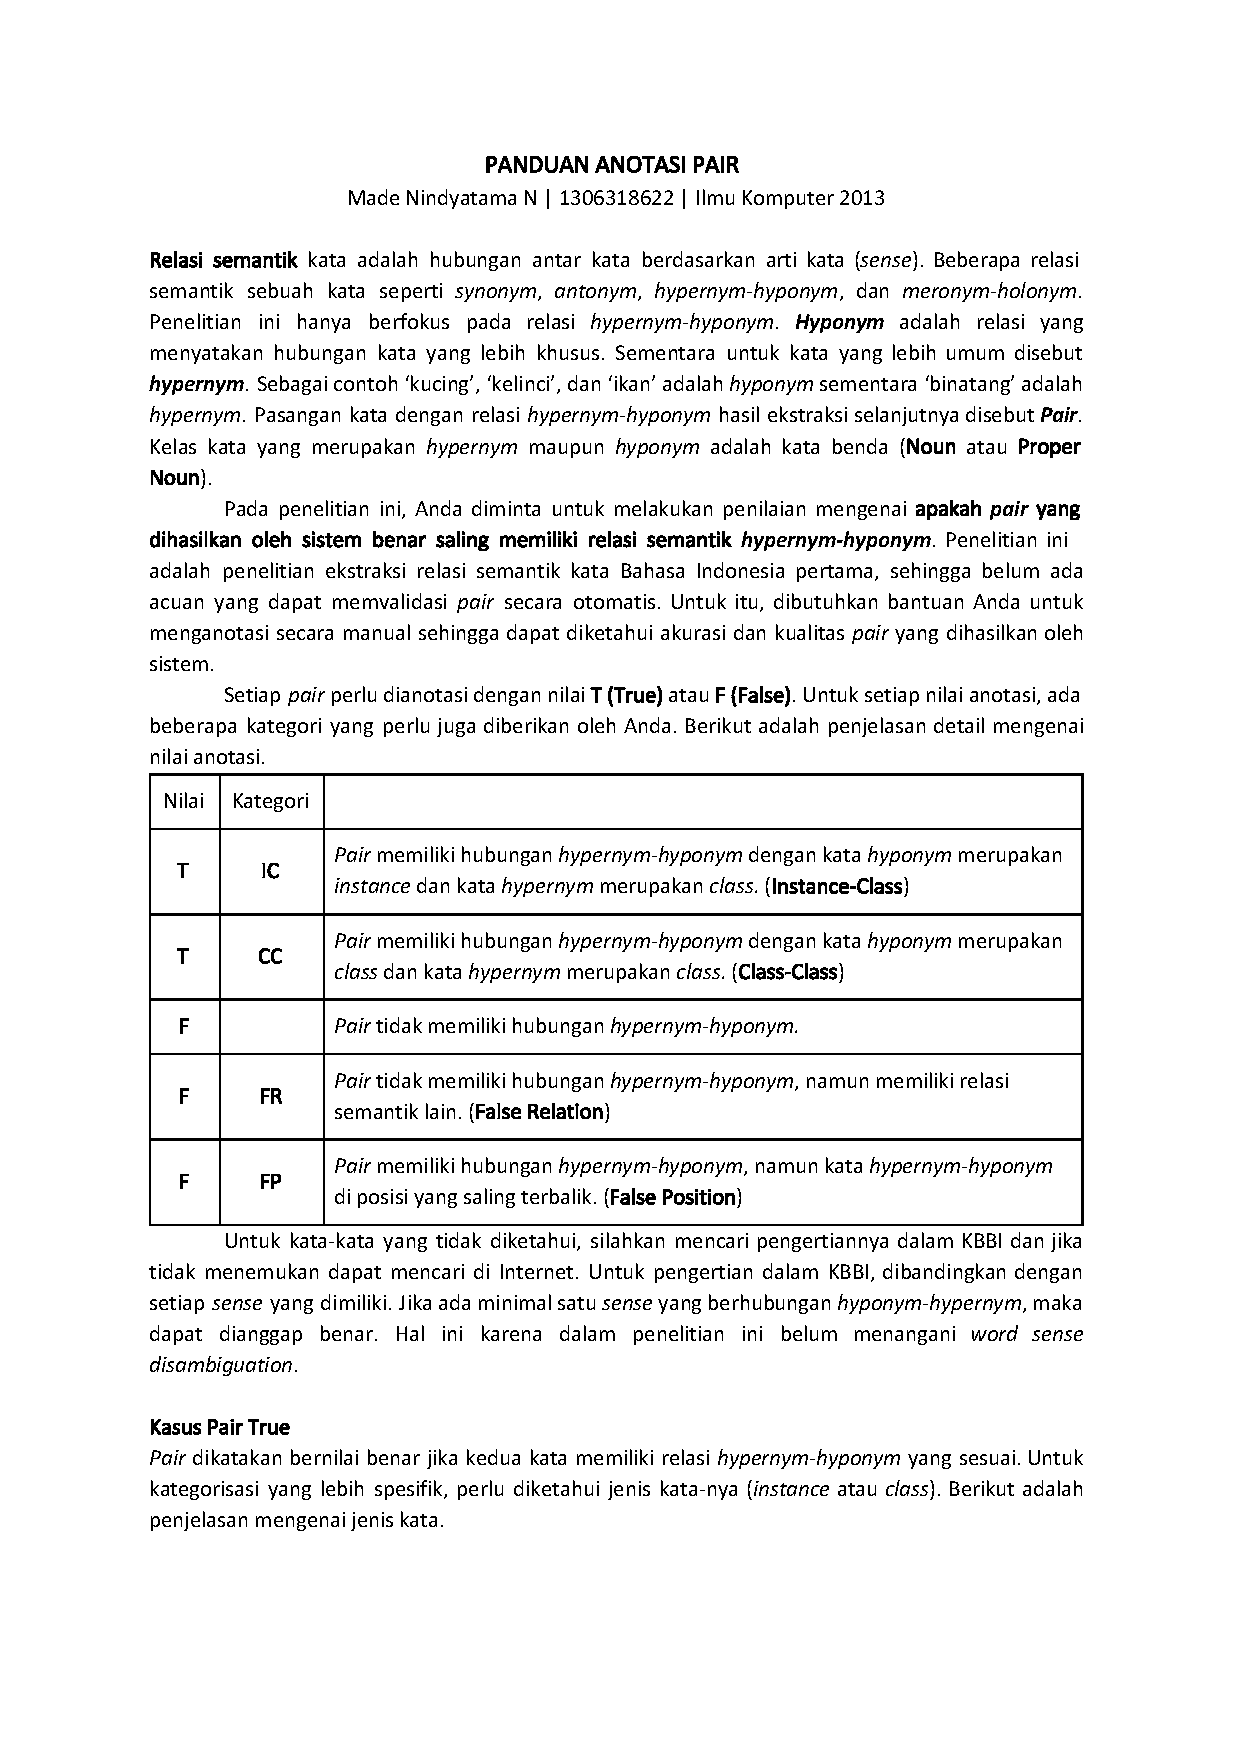
\includepdf[pages={1}]{PanduanAnotasiPair.pdf}
\includepdf[pages={2}]{PanduanAnotasiPair.pdf}
\includepdf[pages={3}]{PanduanAnotasiPair.pdf}

% \section*{\code{admin\_useraddmaster}} \label{cha:lampir-admin}
% Skrip ini diletakkan pada direktori \co{/usr/sesuatu} dan hanya dapat dieksekusi oleh \f{root}. Skrip ini berguna untuk menambahkan pengguna baru sesuai dengan konfigurasi baru yang telah ditetapkan.
% \begin{lstlisting}[style=L,caption={Skrip menambahkan pengguna baru},label={lst:adduser}]
% #!/bin/csh -f
% blah blah blah
% blah blah blah
% blah blah blah
% blah blah blah
% blah blah blah
% \end{lstlisting}

% \section*{\code{getuser.cron}} \label{cha:lampir-cronadmin}
% Penjelasan skrip disini
% \begin{lstlisting}[style=L,caption={\f{Cronjob} menambahkan pengguna baru},label={lst:cronadduser}]
% #!/bin/bash
% # Change these two lines to localize to your system:
% # Adapted from /usr/local/sbin/admin_useradd

% cat /dev/null > $userlist
% for (( i=0; i<${#listemailto[@]}; i++ ))
% do
%         uname=${listusername[$i]}
%         mailto=${listemailto[$i]}

%         echo "User $uname created, please use torqace wisely." | mail -s "Torqace user registration" $mailto
% done

% \end{lstlisting}
% 
% %-----------------------------------------------------------------------------%
% \addChapter{Lampiran 2 : Berkas Konfigurasi}
% \chapter*{Lampiran 2 : Berkas Konfigurasi}
% %-----------------------------------------------------------------------------%
% \section*{compute.xml}
% \begin{lstlisting}[caption={Berkas \co{compute.xml}},label={lst:excomp},language=XML]
% <?xml version="1.0" standalone="no"?>
% <kickstart>
% <description>
% 	Compute node XML file
% </description>
% </kickstart> 
% \end{lstlisting}

% %-----------------------------------------------------------------------------%
% \addChapter{Lampiran 8 : UAT dan Kuesioner}
% %-----------------------------------------------------------------------------%
% \begin{landscape}
% \chapter*{Lampiran 8 : UAT dan Kuesioner}
% \begin{longtable}{|c|p{7cm}|p{2.5cm}|p{3.5cm}|p{3.3cm}|p{1.8cm}|}
% \caption{Tabel UAT dan Kuesioner} \label{tab:uattbl}\\
% \hline
% No. & \multicolumn{1}{c|}{Langkah Penggunaan} & Fitur Berjalan & Tingkat Kemudahan (1-5) & Tingkat Kepuasan (1-5) & Saran / Komentar \\ 
% \cline{3-5} & & Berhasil /Tidak & 1:Sangat sulit ; \hspace{100pt} 5:sangat mudah & 1 : Sangat kecewa ; 5 : sangat puas &  \\ \hline
% \multicolumn{ 6}{|>{\columncolor{headertbl}}c|}{Use Case : Login} \\ \hline
% 1.1 & Pengguna berada pada halaman depan torqace &  &  &  &  \\ \hline
% 1.2 & Pengguna memasukkan username dan password pada field yang telah disediakan.Kemudian menekan tombol 'login' &  &  &  &  \\ \hline
% 1.3 & Apabila Sukses, maka pengguna masuk ke dalam sistem dan dihadapkan pada menu utama &  &  &  &  \\ \hline
% \multicolumn{ 6}{|>{\columncolor{headertbl}}c|}{Use Case : Register} \\ \hline
% 2.1 & Pengguna berada pada halaman registrasi pengguna torqace &  &  &  &  \\ \hline
% 2.2 & Pengguna memasukkan username,password, dan email pada field yang telah disediakan. Kemudian menekan tombol 'submit' &  &  &  &  \\ \hline
% 2.3 & Sistem akan mengonfirmasi masukan, dan akan mengirimkan email untuk memberitahu pengguna apabila proses pendaftaran telah selesai &  &  &  &  \\ \hline
% \multicolumn{ 6}{|>{\columncolor{headertbl}}c|}{Use Case : Logout} \\ \hline
% 3.1 & Pengguna memilih menu untuk melakukan logout &  &  &  &  \\ \hline
% 3.2 & Sistem akan mengeluarkan pengguna, dan pengguna tidak dapat menggunakan fitur-fitur utama aplikasi &  &  &  &  \\ \hline
% \multicolumn{ 6}{|>{\columncolor{headertbl}}c|}{Use Case : Upload Job Sederhana} \\ \hline
% 4.1 & Pengguna memilih menu upload file/project pada menu utama &  &  &  &  \\ \hline
% 4.2 & Pengguna memilih pilihan 'single file' pada tipe project &  &  &  &  \\ \hline
% 4.3 & Pengguna memilih berkas yang akan diunggah, mengisi label, dan menentukan apakah akan menimpa project sebelumnya dengan nama yang sama atau tidak &  &  &  &  \\ \hline
% 4.4 & Pengguna menekan tombol 'submit' dan mengonfirmasi  &  &  &  &  \\ \hline
% 4.5 & Sistem akan menampilkan informasi terkait berkas yang diupload &  &  &  &  \\ \hline
% \multicolumn{ 6}{|>{\columncolor{headertbl}}c|}{Use Case : Upload Job Compressed} \\ \hline
% 5.1 & Pengguna memilih menu upload file/project pada menu utama &  &  &  &  \\ \hline
% 5.2 & Pengguna memilih pilihan 'compressed files' pada tipe project &  &  &  &  \\ \hline
% 5.3 & Pengguna memilih arsip yang akan diunggah, mengisi label, menentukan akan melakukan make atau tidak dan menentukan apakah akan menimpa project sebelumnya dengan nama yang sama atau tidak &  &  &  &  \\ \hline
% 5.4 & Pengguna menekan tombol 'submit' dan mengonfirmasi  &  &  &  &  \\ \hline
% 5.5 & Sistem akan menampilkan informasi terkait berkas yang diupload dan diekstrak. Keluaran make juga akan ditampilkan bila dipilih &  &  &  &  \\ \hline
% \multicolumn{ 6}{|>{\columncolor{headertbl}}c|}{Use Case : Upload Array Job} \\ \hline
% 6.1 & Pengguna memilih menu upload file/project pada menu utama &  &  &  &  \\ \hline
% 6.2 & Pengguna memilih pilihan 'array' pada tipe project &  &  &  &  \\ \hline
% 6.3 & Pengguna memilih arsip-arsip yang akan diunggah, mengisi label, menentukan akan melakukan make atau tidak dan menentukan apakah akan menimpa project sebelumnya dengan nama yang sama atau tidak &  &  &  &  \\ \hline
% 6.4 & Pengguna menekan tombol 'submit' dan mengonfirmasi  &  &  &  &  \\ \hline
% 6.5 & Sistem akan menampilkan informasi terkait berkas yang diupload dan diekstrak. Keluaran make juga akan ditampilkan bila dipilih &  &  &  &  \\ \hline
% \multicolumn{ 6}{|>{\columncolor{headertbl}}c|}{Use Case : Melihat antrian pada queue} \\ \hline
% 7.1 & Pengguna memilih menu  queue status pada menu utama &  &  &  &  \\ \hline
% 7.2 & Pengguna berada pada halaman yang berisi informasi queue &  &  &  &  \\ \hline
% \multicolumn{ 6}{|>{\columncolor{headertbl}}c|}{Use Case : Melihat detil antrian} \\ \hline
% 8.1 & Dari halaman status queue, pengguna memilih job tertentu &  &  &  &  \\ \hline
% 8.2 & Informasi mengenai detil job tersebut ditampilkan dalam bentuk tabel &  &  &  &  \\ \hline
% 8.2.1 & Apabila job tersebut bukan milik pengguna, maka sistem akan melarang pengguna melihat informasi detil suatu job &  &  &  &  \\ \hline
% \multicolumn{ 6}{|>{\columncolor{headertbl}}c|}{Use Case : Membuat script job} \\ \hline
% 9.1 & Pengguna memilih untuk melakukan 'generate script' baik dari laporan upload berkas, atau dari penjelajahan direktori &  &  &  &  \\ \hline
% 9.2 & Pengguna mengisi nama job, parameter job, dan script yang akan dijalankan.  &  &  &  &  \\ \hline
% 9.3 & Pengguna mengonfirmasi konfirmasi submit job &  &  &  &  \\ \hline
% 9.4 & Pengguna dapat melihat informasi script secara keseluruhan dan pesan apakah terjadi kegagalan atau tidak, serta id job yang diberikan &  &  &  &  \\ \hline
% \multicolumn{ 6}{|>{\columncolor{headertbl}}c|}{Use Case : Load spesifikasi job lain} \\ \hline
% 10.1 & Pengguna berada pada halaman untuk membuat script &  &  &  &  \\ \hline
% 10.2 & Pengguna memilih 'Load a Previous Job' &  &  &  &  \\ \hline
% 10.3 & Pengguna memilih job mana yang akan dimuat dan menekan tombol 'Load' &  &  &  &  \\ \hline
% 10.4 & Pengguna kembali ke halaman pembuatan script dengan spesifikasi job sebelumnya &  &  &  &  \\ \hline
% \multicolumn{ 6}{|>{\columncolor{headertbl}}c|}{Use Case : Menjelajah Direktori} \\ \hline
% 11.1 & Pengguna memilih menu  'View File/Project'  pada menu utama &  &  &  &  \\ \hline
% 11.2 & Pengguna dapat melakukan navigasi untuk masuk ke dalam direktori tertentu, atau kembali ke direktori diatasnya, dan dapat melihat terdapat berkas apa saja dalam direktori &  &  &  &  \\ \hline
% \multicolumn{ 6}{|>{\columncolor{headertbl}}c|}{Use Case : Menghapus Berkas/Direktori} \\ \hline
% 12.1 & Pengguna berada pada halaman penjelajahan direktori &  &  &  &  \\ \hline
% 12.2 & Pengguna memilih pilihan untuk menghapus berkas/direktori di samping item yang akan dihapus &  &  &  &  \\ \hline
% 12.3 & Pengguna mengonfirmasi konfirmasi penghapusan &  &  &  &  \\ \hline
% \multicolumn{ 6}{|>{\columncolor{headertbl}}c|}{Use Case : Mengunduh Berkas/Direktori} \\ \hline
% 13.1 & Pengguna berada pada halaman penjelajahan direktori &  &  &  &  \\ \hline
% 13.2 & Pengguna memilih pilihan untuk mengunduh berkas/direktori di samping item yang akan dihapus &  &  &  &  \\ \hline
% \multicolumn{ 6}{|>{\columncolor{headertbl}}c|}{Use Case : Melihat Berkas} \\ \hline
% 14.1 & Pengguna berada pada halaman penjelajahan direktori &  &  &  &  \\ \hline
% 14.2 & Pengguna memilih berkas yang berupa berkas teks &  &  &  &  \\ \hline
% 14.3 & Sistem akan menampilkan konten dari berkas tersebut &  &  &  &  \\ \hline
% \end{longtable}
% \end{landscape}

%\end{appendix}

\end{document}